% Compile with pdflatex report.tex -o report.pdf --mathjax
% Compile each section with pandoc "Vulnerabilities/Path <num>/<vuln>/README.md" -o README.tex

\documentclass{article}
\usepackage[a4paper, margin=1in]{geometry}
\usepackage{fancyhdr}
\usepackage{sectsty}
\usepackage{titlesec}
\usepackage{graphicx}
\usepackage{amsmath}
\usepackage{amssymb}
\usepackage{tikz}
\usepackage{enumerate}

\setlength{\parindent}{0pt} % Remove paragraph indenting

% Define header
\title{\textbf{CITS3006 Project Task 1}}
\author{
    Senaya Wimalasena (24670672)\\
    Dhul Ratnayaka Ratnayaka Mudiyanselage (24518484)\\
    Zarin Tasnim (24315214)\\
    Mohammad Haddadpour (24443565)\\
    Isaac Rutter (24273992)
}
\date{}

% Add page numbers to pages
\pagestyle{fancy}
\fancyhf{}
\fancyfoot[R]{\thepage}                         % Add page numbers (right-aligned)
\fancypagestyle{plain}{\fancyfoot[R]{\thepage}} % Right align page numbers for first page

% Set tag properties
\sectionfont{\fontsize{11}{12}\selectfont}  % \section font properties
\titlespacing*{\section}{0pt}{*0}{0pt}      % \section spacing properties
\titlespacing*{\subsection}{0pt}{0pt}{0pt}  % \subsection spacing properties
\subsectionfont{\fontsize{9}{0}\selectfont} % \subsection font properties
\setlength{\parskip}{1em}                   % \par size
\renewcommand{\headrulewidth}{0pt}          % removes header from fancy page

% Set tikz library properties
\usetikzlibrary{automata, positioning, arrows}
\tikzset{accepting/.style={accepting by double, double distance=1.8pt}}

\begin{document}
    \maketitle

    \newpage

    \section*{Introduction}
    [INTRODUCTION]

    The following is the exploit map for our submission. It consists of three
    distinct paths; Path Alpha, Path Bravo, and Path Charlie. Each of these paths
    eventually lead to a vertical privilege escalation to gain a root shell, every
    previous vulnerability in the path to be satisfied before it can be exploited.
    The categories that we believe each vulnerability belongs to is stated in brackets
    underneath its name, so that they can be identified at a glance.

    Note that there are two branches at the start of Path Alpha. This is because
    the next vulnerability in the path (Reverse Engineering) can be accessed by completing
    either the FTP Misconfiguration challenge OR the pair of \texttt{rip} Manipulation and
    Common Modulus Attack (i.e. you can access the next challenge by completing 
    $(\text{FTP}) \ \lor \ (\text{RE} \ \land \ \text{Cryptography})$). This gives some 
    flexibility in how challenges can be completed, as completing both will lead to the 
    same outcome.

    \begin{figure}[h]
        \centering
        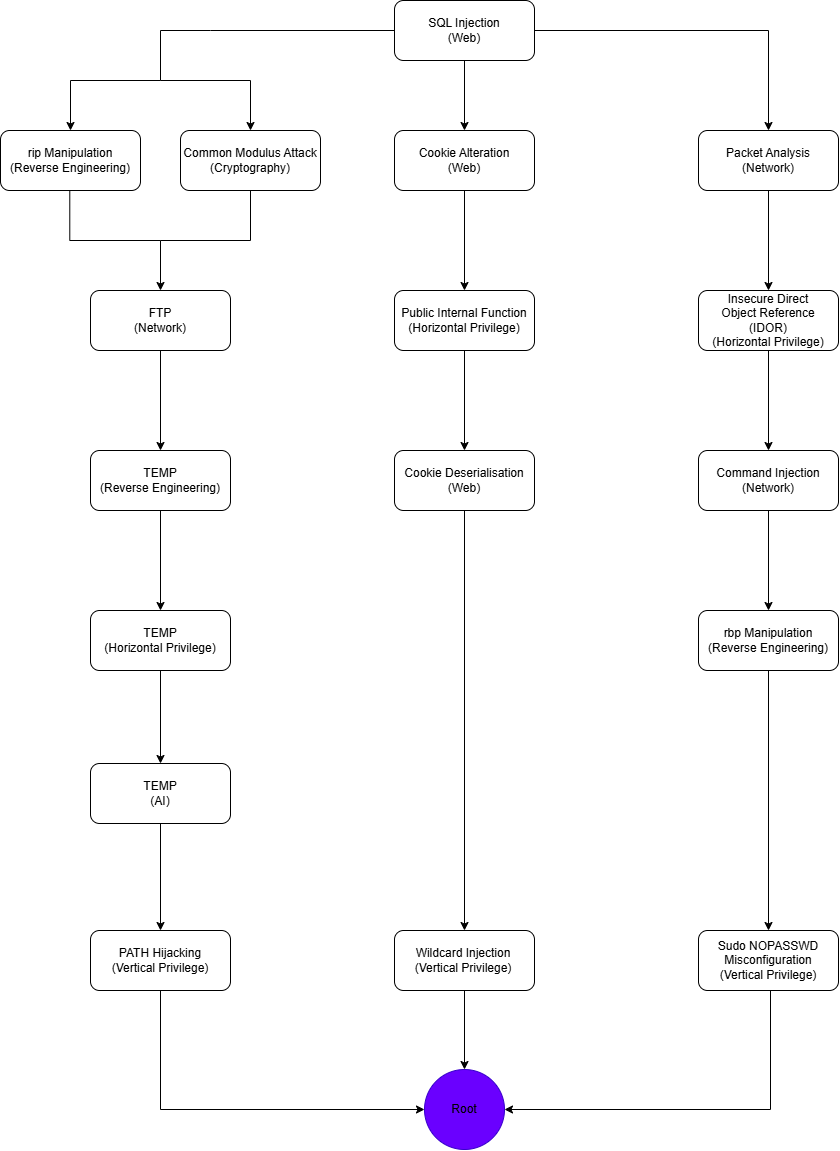
\includegraphics[scale=0.4]{ExploitMap.png}
    \end{figure}

    \newpage

    \section*{SQL Injection (Mohammad + Dhul)}
        Once the application is started, the entry point is located at both
        \texttt{http://localhost:5005} or\\
        \texttt{http://\textless{}container\_IP\textgreater{}:5005}. This will
        bring us to the following web page.
        \begin{center}
            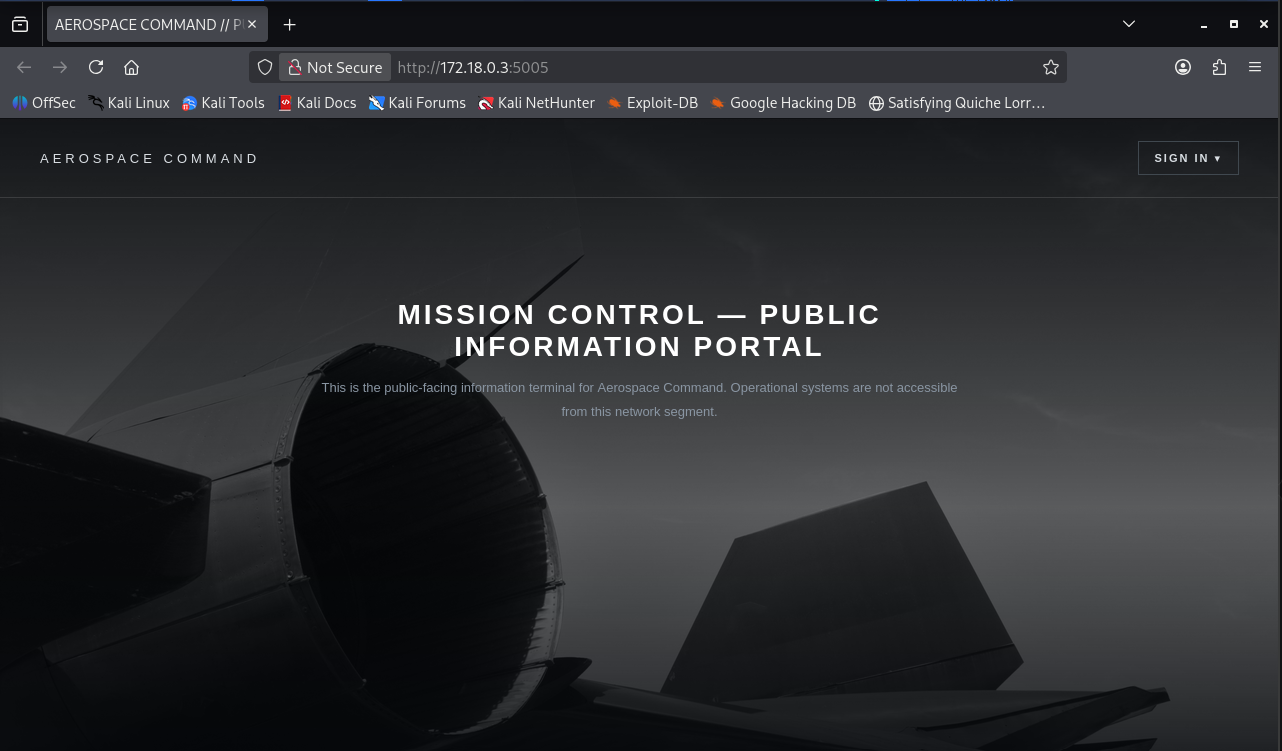
\includegraphics[scale=0.65]{Vulnerabilities/SQLi/images/entry.png}
        \end{center}

        The only option available to us is the ``Sign In'' option in the top
        right. This reveals 2 options - ``Guest Access'' and ``Operator
        Access''. Obviously we want as much privilege as possible, so we will
        try ``Operator Access'' first.
        \begin{center}
            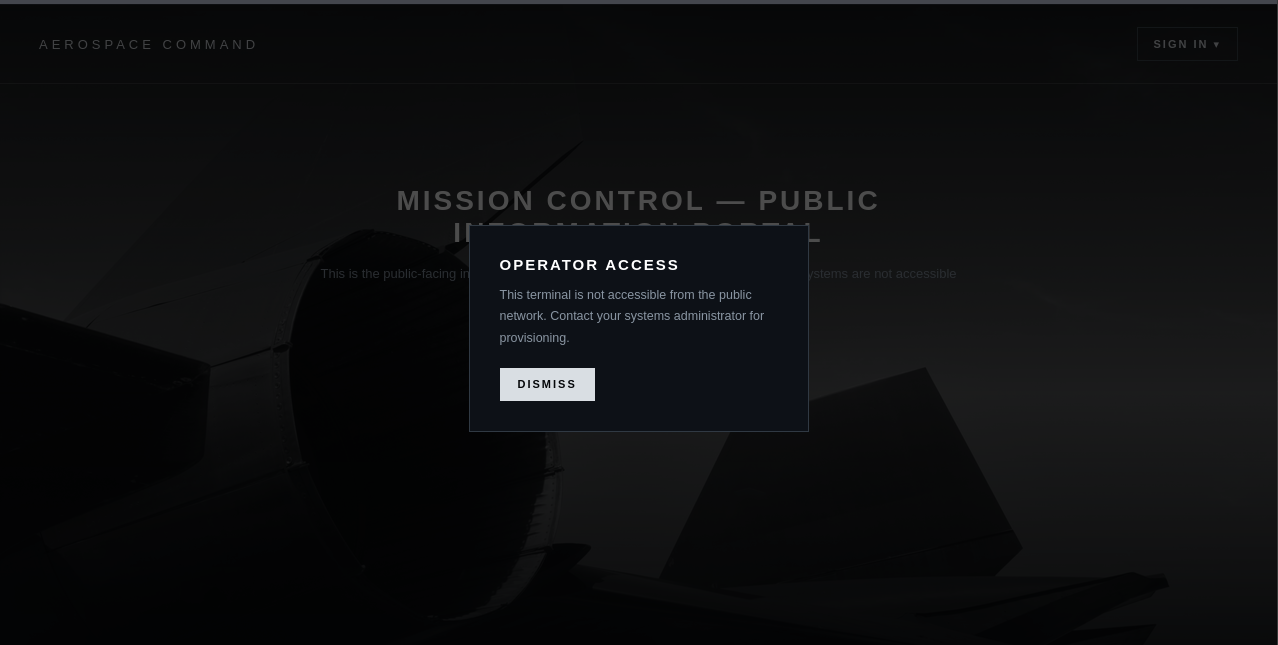
\includegraphics[scale=0.65]{Vulnerabilities/SQLi/images/denial.png}
        \end{center}

        This leads to an error that it cannot be accessed. We should keep this
        in mind for later, but the only option left now is to try ``Guest
        Access''.
        \begin{center}
            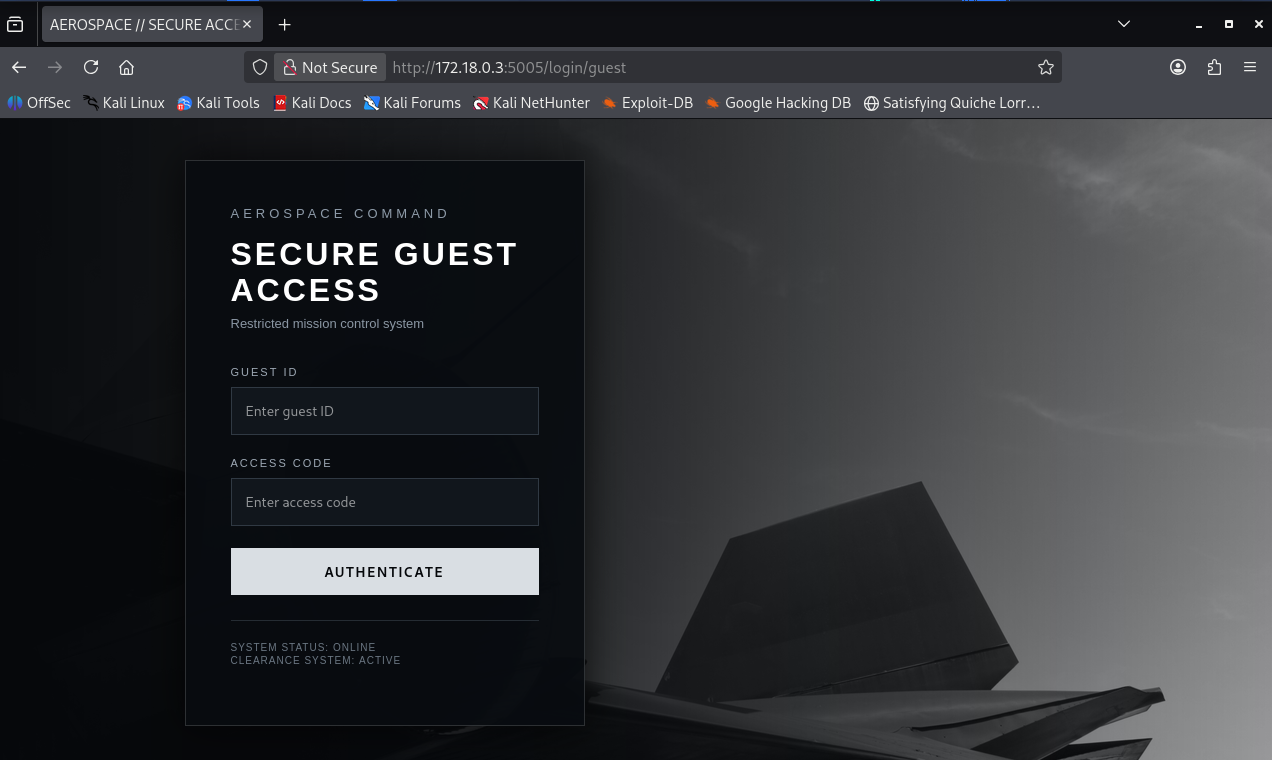
\includegraphics[scale=0.65]{Vulnerabilities/SQLi/images/guest.png}
        \end{center}

        This has led us to a fairly standard login panel. However, we don't know
        any credentials so this must be able to be exploited some other way. The
        URL leads to the path \texttt{/login/guest}, so we can try and access
        the operator panel by navigating to \texttt{/login/operator} and seeing
        if that works.
        \begin{center}
            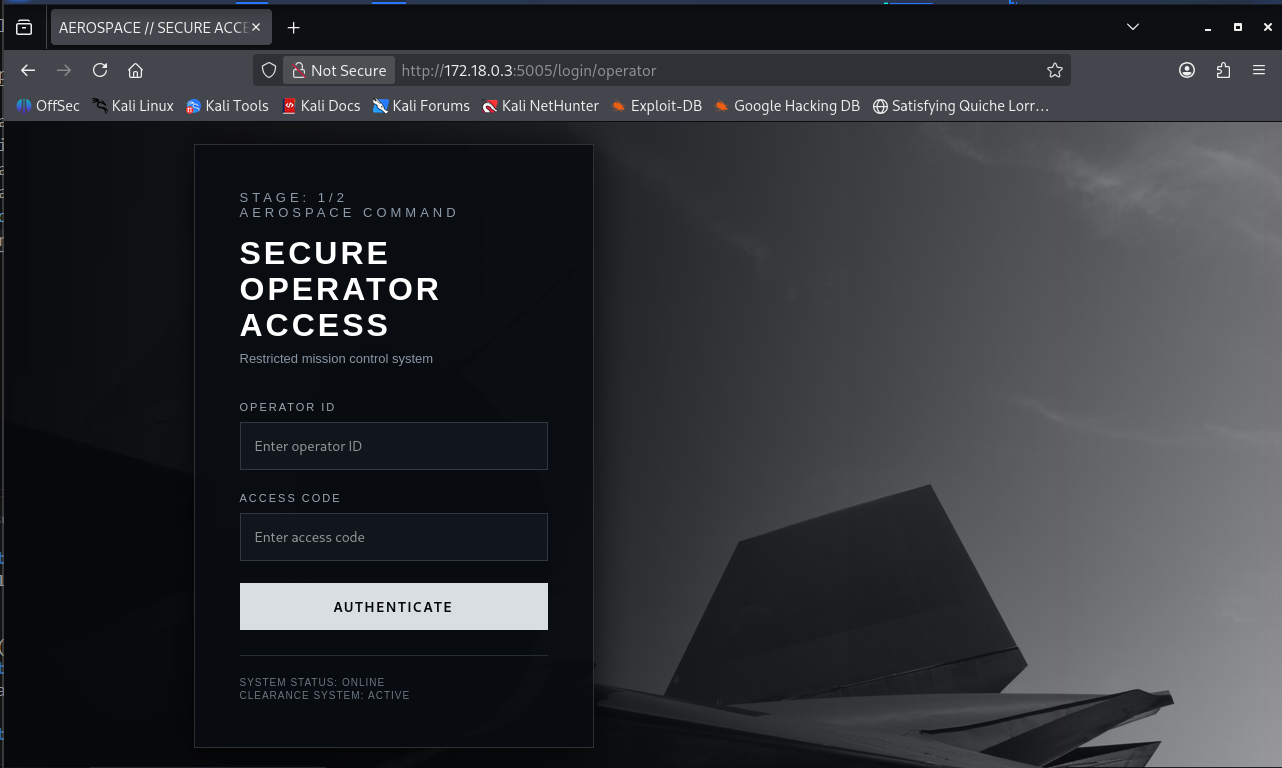
\includegraphics[scale=0.65]{Vulnerabilities/SQLi/images/operator.png}
        \end{center}

        This has led to the operator login panel, which means we are on the
        right track. There are a few things to note here; we need an operator
        ID/access code (likely just a username and password) and this is stage 1
        of 2 apparently. We don't know any credentials yet so we should try to
        enter anything and see what happens.
        \begin{center}
            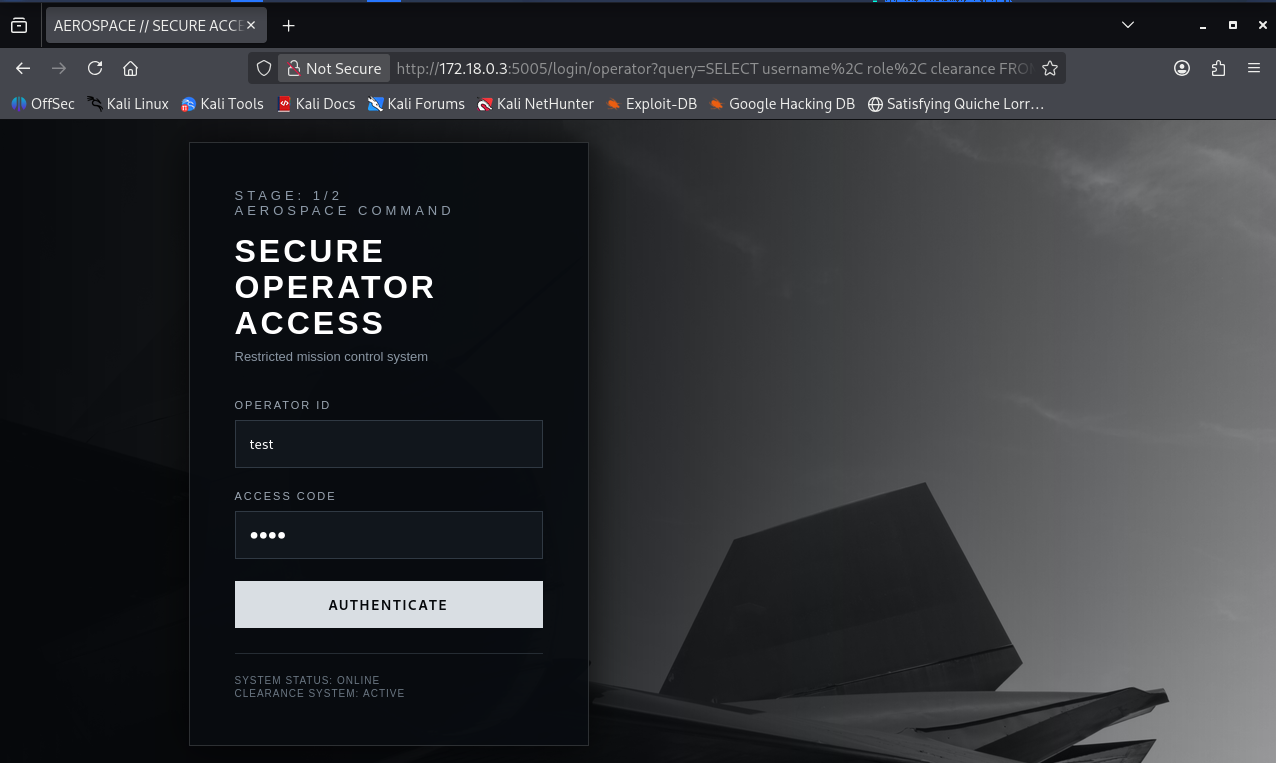
\includegraphics[scale=0.65]{Vulnerabilities/SQLi/images/stage_1.png}
        \end{center}

        Visually this didn't change anything, but the URL changed with a new
        \texttt{query} parameter that appears to be an SQL query
        (\texttt{SELECT\%20username\%2C\%20role\%2C\%20clearance\%20FROM\%20users\%20WHERE\%20\\username\%20\%3D\%20\%27test\%27\%20AND\%20password\%20\%3D\%20\%27test\%27}
        or
        \texttt{SELECT\ username\%2C\ role\%2C\ clearance\ FROM\ users\ WHERE\ username\ \%3D\ \textquotesingle{}test\textquotesingle{}\ AND\ password\ \%3D\ \textquotesingle{}test\textquotesingle{}}
        depending on the browser being used). This is URL encoded, but by
        decoding it we can see the query being executed is
        \texttt{SELECT\ username,\ role,\ clearance\ FROM\ users\ WHERE\ username\ =\ \textquotesingle{}test\textquotesingle{}\ AND\ password\ =\ \textquotesingle{}test\textquotesingle{}}.
        Since we can directly manipulate the query, this seems like the obvious
        solution. As we don't know the password, we can just remove this section
        entirely so that we only have to match the username. We don't know the
        username, but we can probably assume that one of them is \texttt{admin}
        or \texttt{administrator}. We can try this using the URL
        \texttt{http://localhost:5005/login/operator?query=ELECT\%20username\%2C\%20role\\\%2C\%20clearance\%20FROM\%20users\%20WHERE\%20username\%20\%3D\%20\%27admin\%27}.
        \begin{center}
            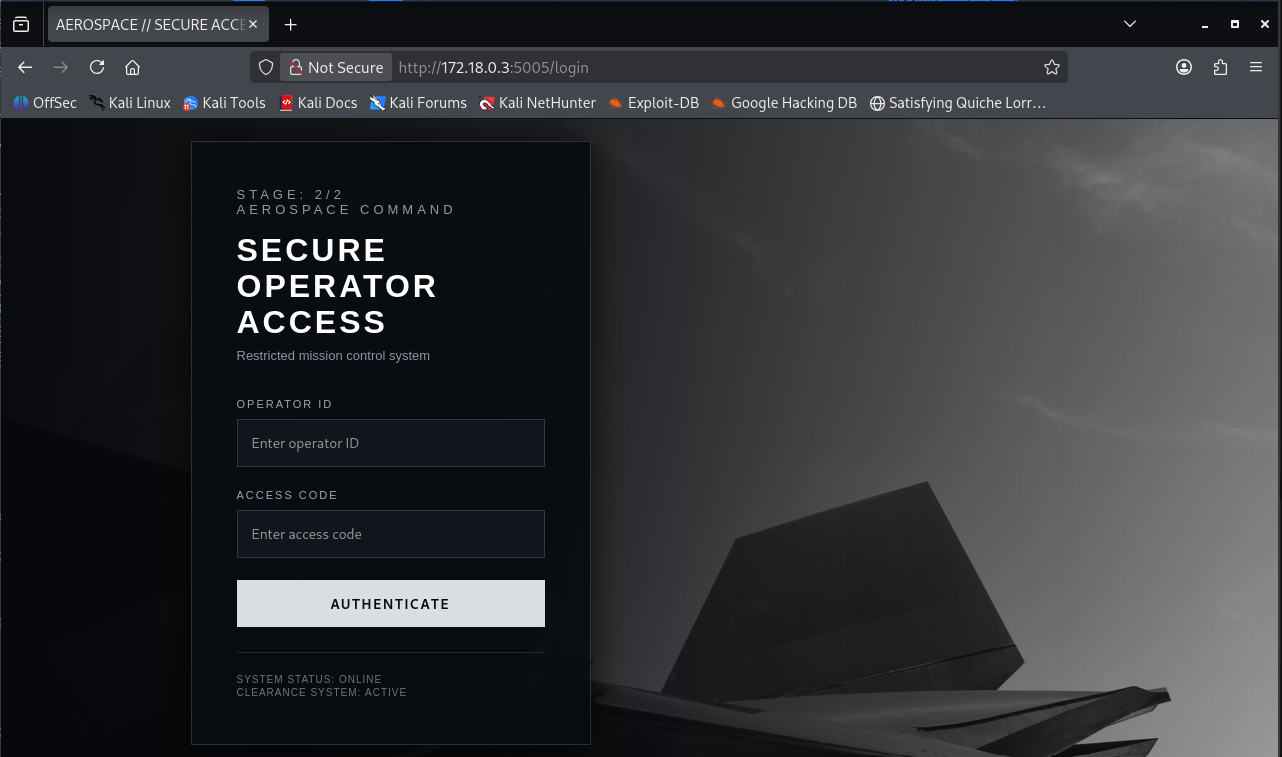
\includegraphics[scale=0.65]{Vulnerabilities/SQLi/images/stage_2.png}
        \end{center}

        This had led to stage 2 of the login panel, indicating that
        \texttt{admin} was, indeed, a valid username. At this point we have no
        further information so we need to test this panel to see if anything
        happens.
        \begin{center}
            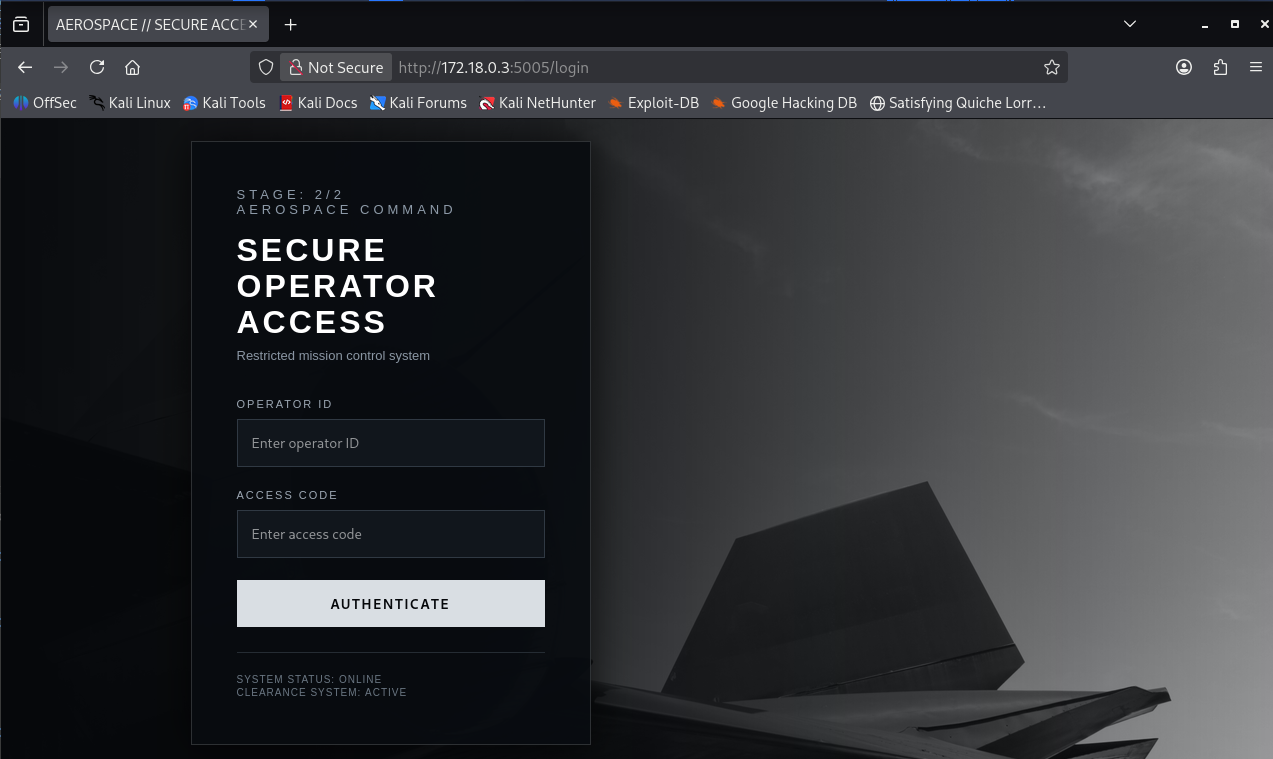
\includegraphics[scale=0.65]{Vulnerabilities/SQLi/images/test_2.png}
        \end{center}

        After entering some test credentials, there are no visual changes to the
        UI or URL so there must be another solution. Even after looking at the
        website's cookies and source code for any potential information, nothing
        can be found. As we have nothing else to work on, we can try to
        construct a basic SQL injection attack. This can be done using
        \texttt{\textquotesingle{}\ OR\ 1=1\ -\/-} as the username to see if
        anything happens.
        \begin{center}
            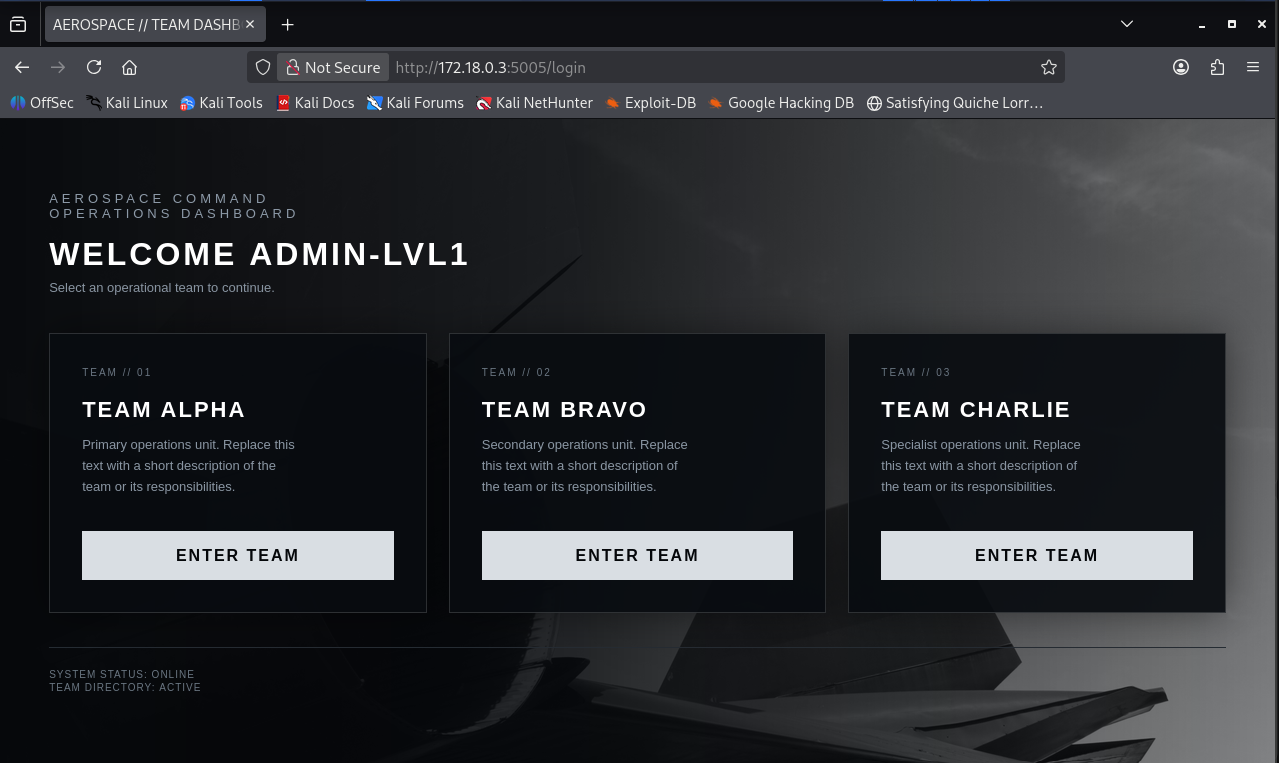
\includegraphics[scale=0.65]{Vulnerabilities/SQLi/images/dashboard.png}
        \end{center}

        This has allowed us to login, showing the dashboard for the web
        application. The dashboard has three different ``categories''; Team
        Alpha, Team Bravo, and Team Charlie. Each of these correspond to one of
        the three exploit paths, so we will visit these in order.

    \newpage

    \section*{Path Alpha}
    Entering the Team Alpha section will lead to the following page:
    \begin{center}
        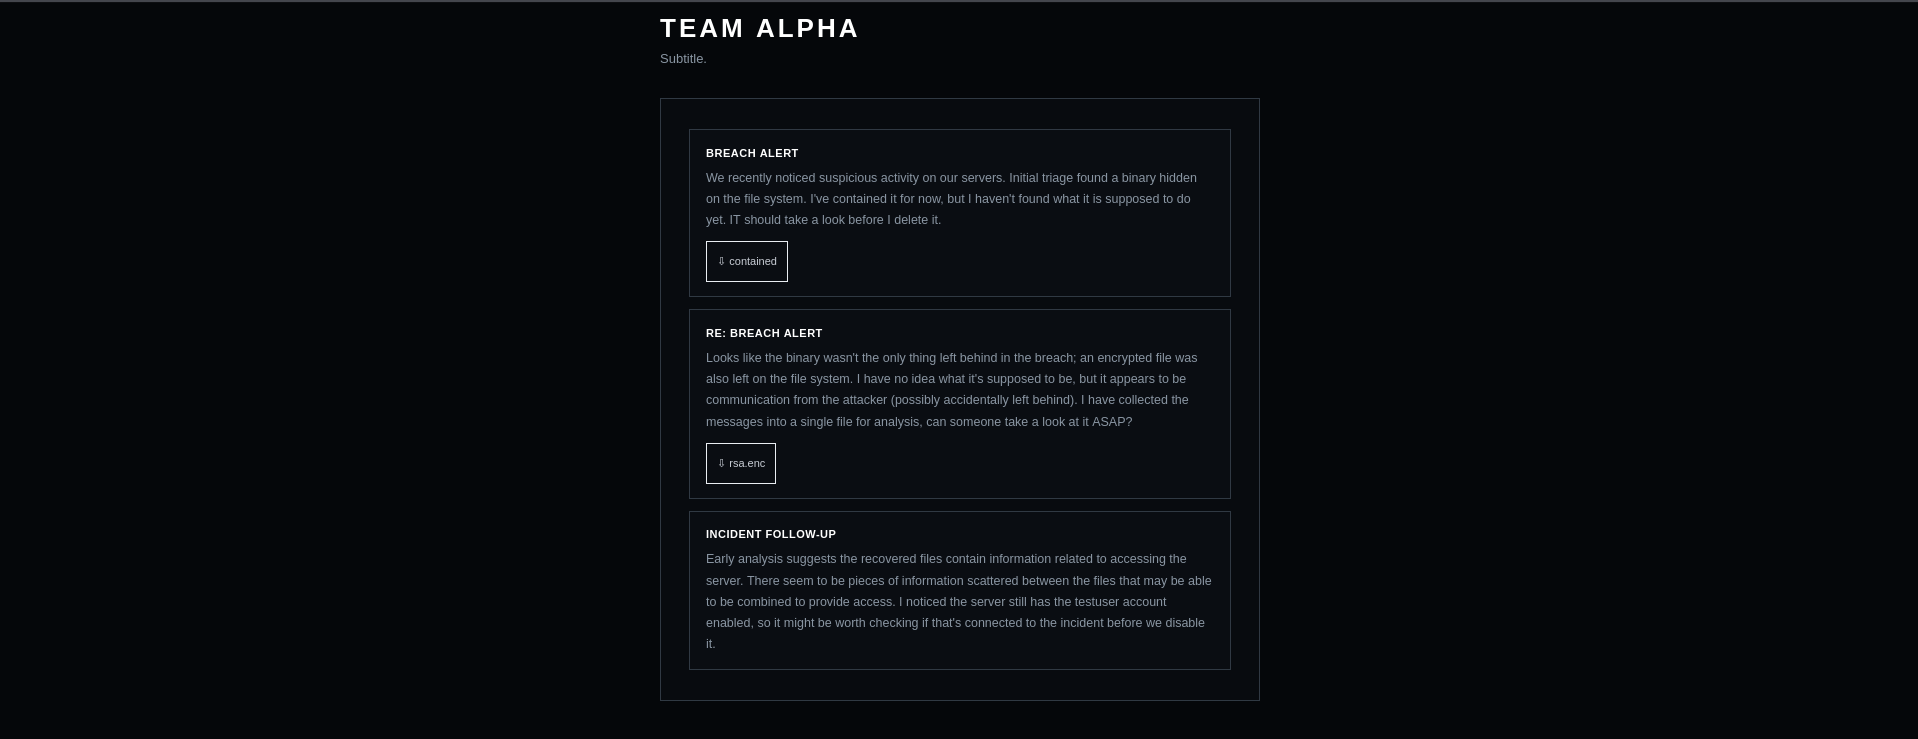
\includegraphics[scale=0.45]{Vulnerabilities/images/alpha.png}
    \end{center}

    This includes two downloadable files; \texttt{contained}, which is necessary for the
    reverse engineering challenge, and \texttt{rsa.enc}, which is necessary for the
    cryptography challenge. These can both be downloaded to the local system to complete
    the associated challenges.

    \vspace{1em}

    \subsection*{\texttt{rip} Manipulation (Isaac)}
        This vulnerability only requires \texttt{gef}, but \texttt{strings} and
        \texttt{ghidra} may be useful too.

        To begin, the binary can be inspected using \texttt{file\ re} to gain
        some information about its structure and how it was compiled since this
        could give us an indication of how it is vulnerable.
        \begin{center}
            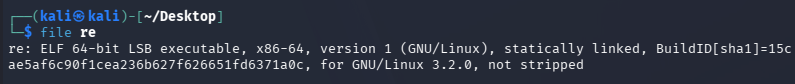
\includegraphics[keepaspectratio,alt={file}]{Vulnerabilities/Path 1/RE/images/file.png}
        \end{center}

        The binary seems to be pretty standard. The only notable aspects are
        that it is statically linked and not stripped, which could be exploited.
        However, we need more information. To see what the binary actually does,
        we can run it and see what happens.
        \begin{center}
            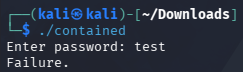
\includegraphics[keepaspectratio,alt={run}]{Vulnerabilities/Path 1/RE/images/run.png}
        \end{center}

        The binary asks for a password, and since we don't know what it is
        returns failure. It is possible that the password has just been written
        in plaintext in the binary, so we can dump the strings from the binary
        to investigate. However, as the binary is statically linked, there is a
        lot of noise in the binary. This dumps the strings from every single
        library that has been compiled with the binary, which makes it hard to
        determine what is unique to the binary and what was from a library. As
        such, we need to take another approach. Using a debugger like
        \texttt{gef} seems like the obvious next step, so we can try that. The
        obvious thing to do would be to see what the \texttt{main} function
        does, so that can be disassembled.
        \begin{center}
            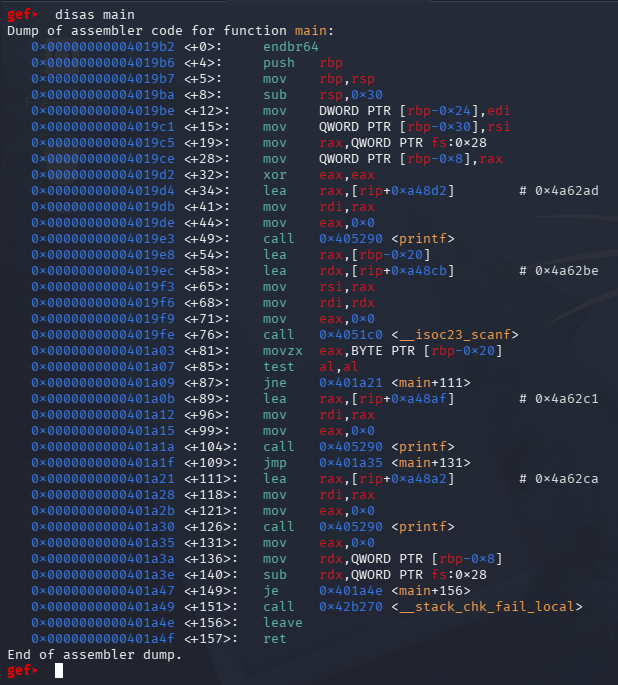
\includegraphics[scale=0.65]{Vulnerabilities/Path 1/RE/images/main.png}
        \end{center}

        From this disassembly, there doesn't seem to be anything of note.
        There's only a \texttt{scanf} call and 2 \texttt{printf} calls (both of
        which have already been seen) but nothing immediately jumps out. There
        does seem to be a comparison at some point with the \texttt{je}
        instruction, but no obvious comparison values. As there is nothing else
        to go on, seeing what functions are in the program might be helpful -
        nothing is called by \texttt{main()}, but that doesn't mean that there
        isn't anything that could give a hint to the solution.
        \begin{center}
            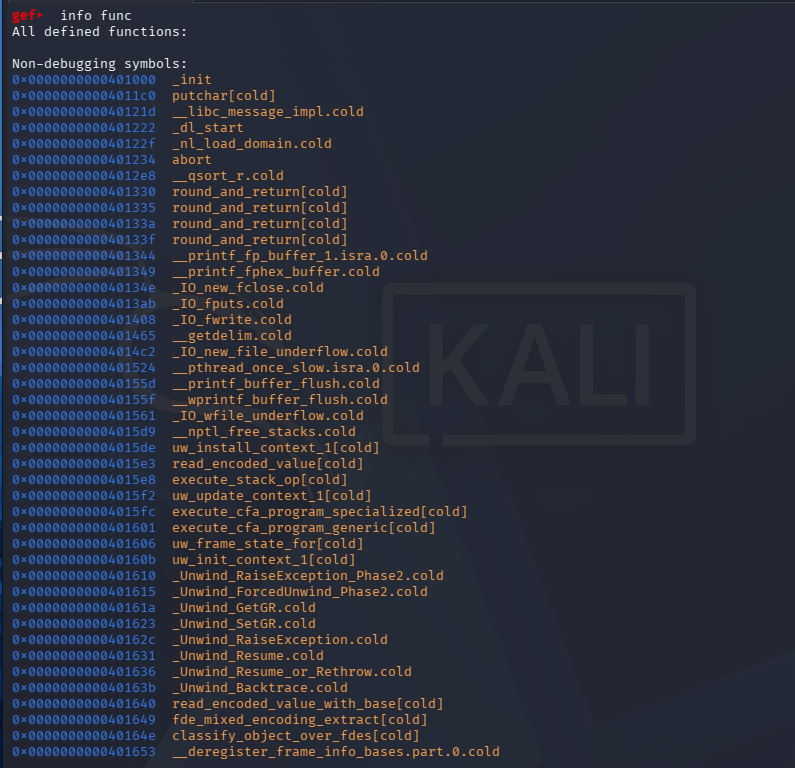
\includegraphics[scale=0.65]{Vulnerabilities/Path 1/RE/images/functions.png}
        \end{center}

        The program, as expected, has a lot of functions due to the previously
        identified static linking. However, after going through the whole list,
        there is one function that stood out - \texttt{get\_flag()}. This is not
        part of any library and not called by \texttt{main} so its purpose isn't
        clear, but it's worth investigating. For now, disassembling it seems
        like the natural next step.
        \begin{center}
            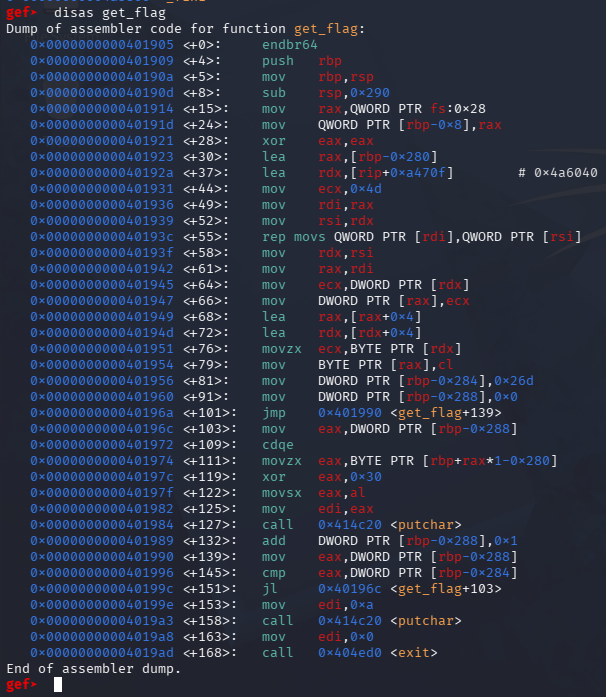
\includegraphics[scale=0.65]{Vulnerabilities/Path 1/RE/images/flag.png}
        \end{center}

        This function seems to be doing quite a bit more work than
        \texttt{main}. There are some \texttt{putchar} function calls, which
        seems like a natural place for the flag to be. Although this function is
        not called from \texttt{main}, it doesn't need to be. The \texttt{rip}
        register, which stores the address for the next instruction to execute,
        can be directly manipulated using \texttt{gef}. By setting \texttt{rip}
        to the start of this function, we can execute the function and see what
        it does.
        \begin{center}
            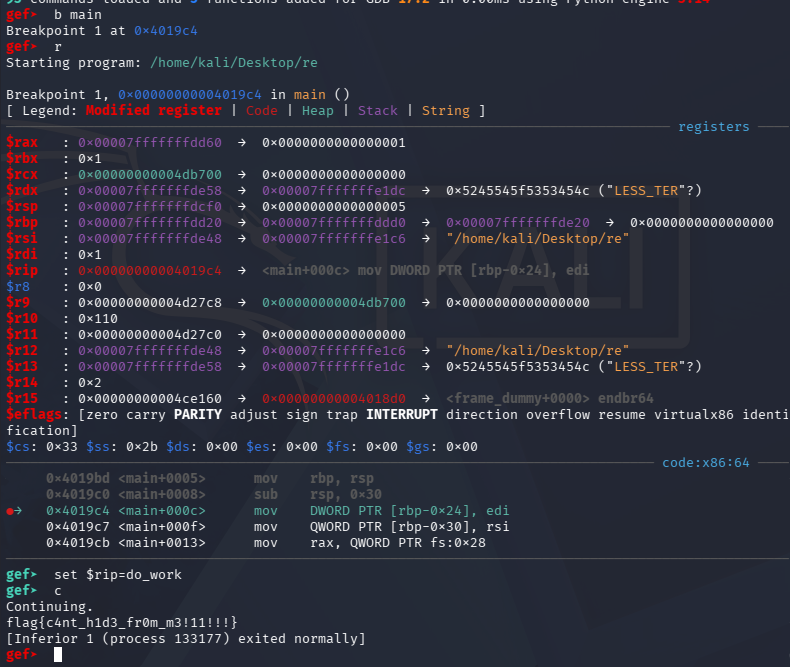
\includegraphics[scale=0.65]{Vulnerabilities/Path 1/RE/images/rip.png}
        \end{center}

        This prints the flag immediately with no other work required. This
        function would have never been found without reverse engineering it, so
        this binary has been completely reverse engineered.

    \vspace{1em}

    \subsection*{Common Modulus RSA Attack (Isaac)}
        For this task, the only thing that is provided is \texttt{rsa.enc},
        which looks like the following.
        \begin{verbatim}
        n1 = 608274...712081

        c1 = 201700...036721

        e1 = 3

        n2 = 608274...712081

        c2 = 297771...598737

        e2 = 5
        \end{verbatim}

        This includes 6 different values; \texttt{n1}, \texttt{c1},
        \texttt{e1}, \texttt{n2}, \texttt{c2}, and \texttt{e2}. The file name
        including \texttt{rsa} indicates that we are dealing with the RSA
        encryption algorithm, which means we know what each of these values
        represent. \texttt{c} is the ciphertext which we are trying to convert
        into plaintext, and \texttt{n} and \texttt{e} are the public key
        components. As there is nothing else to work on, we can assume that the
        goal is to convert the ciphertext (\texttt{c}) into plaintext
        (\texttt{m}).

        One of the first things to notice about these values is that there is a
        red herring; \texttt{n1} and \texttt{n2} are the same value. This is
        important information because it narrows down what we can do with these
        values. However, given that we have two different ciphertexts with the
        same modulus \texttt{n}, it can be assumed that we are going to perform
        a common modulus attack. As \texttt{e1} and \texttt{e2} are specifically
        coprime, this possibility becomes even more likely.

        Bezout's theorem can be used to decrypt the ciphertext to retrieve the
        plaintext message. As we know that \texttt{e1} and \texttt{e2} are
        coprime, then \texttt{gcd(e1,\ e2)\ =\ 1}. By Bezout's theorem, this can
        be used to compute \texttt{m} from \texttt{c1} and \texttt{c2}.

        \begin{verbatim}
        from math import gcd

        n = 608274...712081
        c1 = 201700...036721
        e1 = 3
        c2 = 297771...598737
        e2 = 5
        
        # Adapted from https://susanou.github.io/Writeups/posts/RSA-Common-Modulus/
        s1 = pow(e1, -1, e2)
        s2 = (gcd(e1, e2) - e1*s1)//e2
        temp = pow(c2, -1, n)
        m1 = pow(c1, s1, n)
        m2 = pow(temp, -s2, n)
        print((m1 * m2) % n)
        \end{verbatim}

        This results in the following value.

        \begin{verbatim}
        248553018214215493487040500207679911872168453218024546771910211720
        406762531126531703938858752533393106709772827557749049521555884150
        604259193594527423259444784382279526552592511932044342078635300729
        270182794399218532493518987097151611922743079927408121530187350545
        118718450517411631183686866066732804662224083035106567473238166691
        830868904475417848555088722856249916463283456430566876009997435073
        449383683873658844053220605377161746406258446444675544777485779366
        541092562042762820615071010338311013119161809328197454123675748485
        638053194585907067815386257709049773415511650831052108606440355750
        96141973536633499558383
        \end{verbatim}

        Using the other value gained from the previous challenge, we can now
        move onto the next challenge.

    \vspace{1em}

    \subsection*{FTP Misconfiguration (Dhul)}

    \vspace{1em}

    \subsection*{Reverse Engineering (Mohammad)}

    \vspace{1em}

    \subsection*{Horizontal Privilege (Senaya)}

    \vspace{1em}

    \subsection*{AI (Zarin)}

    \vspace{1em}

    \subsection*{\texttt{PATH} Hijacking (Isaac)}
        Now that we have gotten to the new user account, we can see what this
        account has access to. The obvious place to start is to see what files
        exist in their home directories.
        \begin{center}
            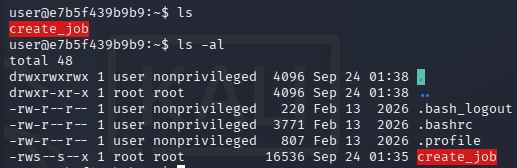
\includegraphics[keepaspectratio,alt={ls}]{Vulnerabilities/Path 1/VPE/images/ls.png}
        \end{center}

        The most interesting thing is a \texttt{create\_job} binary owned by
        root with the setuid bit active which the user can execute. This needs
        to be further explored, so we can see what the binary does for any
        leads.
        \begin{center}
            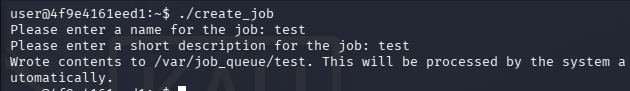
\includegraphics[keepaspectratio,alt={test}]{Vulnerabilities/Path 1/VPE/images/test.png}
        \end{center}

        There are two useful things that can be identified from the output of
        the program. First, it looks like it takes a name for a job and a
        description and writes the contents to
        \texttt{/var/job\_queue/\textless{}job\_name\textgreater{}}. It looks
        like it also is somehow processed by the system automatically. As there
        is nothing else to work with, exploring the directory first seems like
        the natural next step.
        \begin{center}
            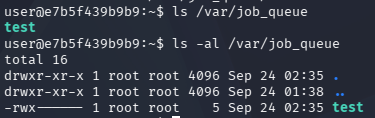
\includegraphics[keepaspectratio,alt={job\_queue}]{Vulnerabilities/Path 1/VPE/images/job_queue.png}
        \end{center}

        It looks like the jobs sent to this queue become owned by root with the
        full \texttt{rwx} permissions. As these are seemingly just text files,
        this is probably a misconfiguration but we can try to exploit this.
        However, this seems like a dead end. As we know that the system
        processes jobs automatically, there must be some background process that
        is run to process these jobs somehow. We can try to identify what this
        process is using \texttt{ps\ aux}, which will list all processes
        currently running on the system.
        \begin{center}
            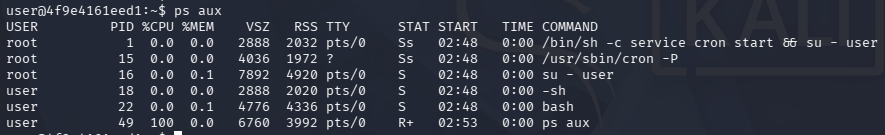
\includegraphics[keepaspectratio,alt={processes}]{Vulnerabilities/Path 1/VPE/images/processes.png}
        \end{center}

        It looks like the system is running a \texttt{cron} job, which is likely
        how these jobs are automatically processed. As \texttt{cron} jobs can be
        stored in different directories in \texttt{/etc}, it is worth
        identifying which directories exist on the system for further
        exploration.
        \begin{center}
            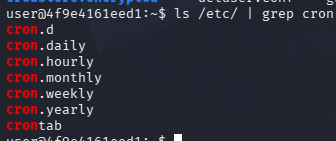
\includegraphics[keepaspectratio,alt={cron\_dirs}]{Vulnerabilities/Path 1/VPE/images/cron_dirs.png}
        \end{center}

        There are a total of 7 different directories that can be searched.
        Naturally, going in order (so starting with \texttt{cron.d}) makes the
        most sense.
        \begin{center}
            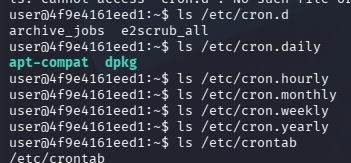
\includegraphics[keepaspectratio,alt={cron\_ls}]{Vulnerabilities/Path 1/VPE/images/ls_cron.png}
        \end{center}

        The only directories that have contents are \texttt{cron.d} and
        \texttt{cron.daily}. However, \texttt{cron.daily} includes standard
        Ubuntu jobs leaving only \texttt{cron.d}. This includes an
        \texttt{archive\_jobs} file, which sounds like exactly what we need.
        Therefore, this is our next target.
        \begin{center}
            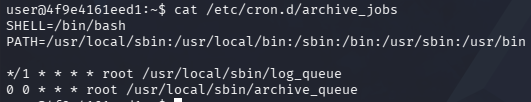
\includegraphics[keepaspectratio,alt={cron\_jobs}]{Vulnerabilities/Path 1/VPE/images/cron_jobs.png}
        \end{center}

        This file lists two jobs - a \texttt{log\_queue} job which runs once
        every minute and an \texttt{archive\_queue} job which runs every day at
        midnight (0:00). These jobs both run as root, which could be the way
        that we achieve a root shell. Before it can be decided how to approach
        this, both scripts need to be checked for potential vulnerabilities.
        \begin{center}
            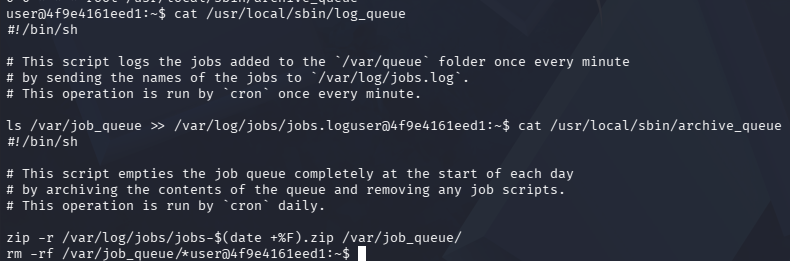
\includegraphics[keepaspectratio,alt={scripts}]{Vulnerabilities/Path 1/VPE/images/scripts.png}
        \end{center}

        It appears that both scripts are Bash scripts which are executed by
        \texttt{cron} at designated times to perform specific actions (which
        aren't relevant to what we are doing here). However, there is something
        interesting about these files; they call standard Linux utilities using
        unqualified path names. As we know that the \texttt{create\_job} utility
        has root privileges, we can attempt to create a job that has custom
        instructions to create a root shell. To do this, we need to check where
        each of the utilities are located to choose a suitable location on the
        \texttt{cron} job's \texttt{PATH} so that our custom utility is the one
        that gets executed. As the first job executes every minute, the binaries
        in this file are our candidates. This script only uses \texttt{ls}, so
        this will be our target binary.
        \begin{center}
            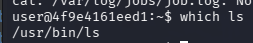
\includegraphics[keepaspectratio,alt={which\_ls}]{Vulnerabilities/Path 1/VPE/images/which_ls.png}
        \end{center}

        It appears that the current \texttt{ls} binary is located at
        \texttt{/usr/bin/ls}. This is at the very end of the \texttt{cron} job's
        \texttt{PATH}, so we can attempt to place it in any other directory on
        the \texttt{PATH}. Arbitrarily, we will use \texttt{/usr/local/sbin} as
        the target destination since this will be found first. As we know the
        files get written to \texttt{/var/job\_queue}, we need to try making it
        write to \texttt{/usr/local/sbin}. As the program has root, it can write
        anywhere with no restrictions. Therefore, we can try and see if
        \texttt{../../usr/local/sbin/ls} will work.
        \begin{center}
            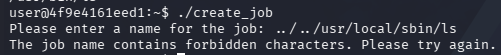
\includegraphics[keepaspectratio,alt={dir\_traversal}]{Vulnerabilities/Path 1/VPE/images/dir_traversal_test.png}
        \end{center}

        This leads to an error that the job name has forbidden characters. To
        see what these forbidden characters are, we need to test it somehow.
        This would take forever trying to work it out manually, so reverse
        engineering the binary makes the most sense since the forbidden
        characters are likely stored inside the binary. To do this, Ghidra will
        be used so we can see the decompiled C code as well which might make
        this easier. This requires the binary to be copied using \texttt{scp} on
        the machine so it can be saved to our host. Once this is done and the
        decompiled binary is inspected, we can identify a few notable
        properties.
        \begin{center}
            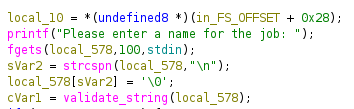
\includegraphics[keepaspectratio,alt={validate\_string}]{Vulnerabilities/Path 1/VPE/images/validate_string.png}
        \end{center}

        The name for the job (and its contents) are checked with the
        \texttt{validate\_string()} function. This can be checked to see what
        characters we aren't allowed to use.
        \begin{center}
            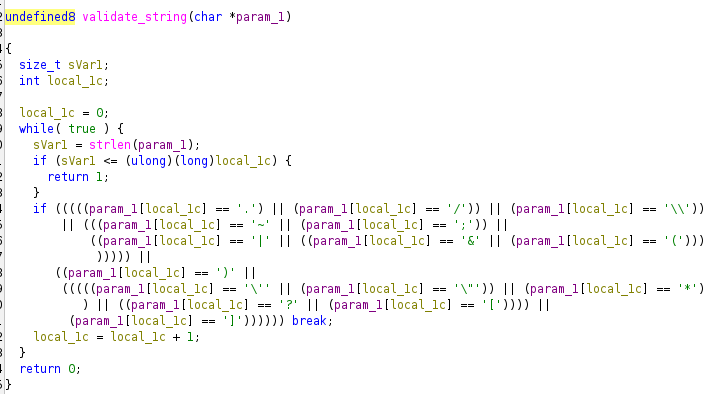
\includegraphics[keepaspectratio,alt={invalid}]{Vulnerabilities/Path 1/VPE/images/invalid_chars.png}
        \end{center}

        From this decompilation, it looks like we can't use \texttt{.},
        \texttt{/}, \texttt{\textbackslash{}},
        \texttt{\textasciitilde{}}, \texttt{;}, \texttt{\textbar{}},
        \texttt{\&}, \texttt{(}, \texttt{)}, \texttt{\textquotesingle{}},
        \texttt{"}, \texttt{*}, \texttt{?}, \texttt{{[}}, or \texttt{{]}}. This
        means that we need some other way to inject them. After going through
        the decompiled code again, we can see how the file is written.
        \begin{center}
            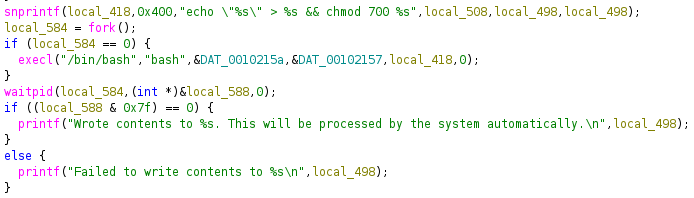
\includegraphics[keepaspectratio,alt={execl}]{Vulnerabilities/Path 1/VPE/images/execl.png}
        \end{center}

        The jobs are written using \texttt{execl} using \texttt{echo} on
        \texttt{bash}. The \texttt{execl} function uses the caller's
        environment, so we might be able to use environment variables to write
        files wherever we want. As we know it uses a \texttt{bash} shell call,
        we know it can expand variables so this is something worth trying. The
        program only checks the unexpanded form, so this should give some sort
        of result. This can be tested using the same example as before, but
        inserting the forbidden characters as environment variables.
        \begin{center}
            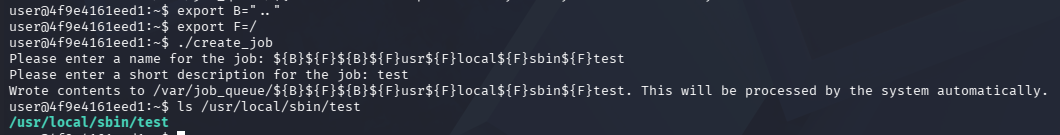
\includegraphics[scale=0.75]{Vulnerabilities/Path 1/VPE/images/env_traversal_test.png}
        \end{center}

        As shown, this has successfully created a file in the
        \texttt{/usr/local/sbin} directory which is normally only writable by
        root. Now that we have a way to write arbitrary information wherever we
        want, we need to construct a payload that will allow us to activate a
        root shell. The only thing we need to do is create a copy of
        \texttt{/bin/bash} that the current user can access and give it the
        setuid bit so that it executes as root. This is a pretty simple Bash
        script, which can be written as the following:

        \begin{verbatim}
        #!/bin/bash
        cp /bin/bash /home/user/bash
        chmod +s /home/user/bash
        \end{verbatim}

        This requires some additional environment variables to be created to get
        around the program's filter, but this is pretty simple to do.
        \begin{center}
            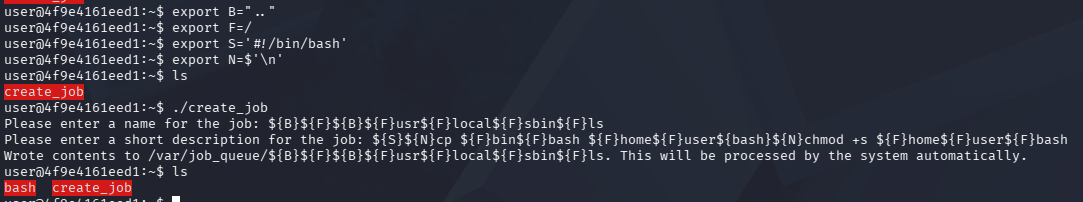
\includegraphics[scale=0.75]{Vulnerabilities/Path 1/VPE/images/payload.png}
        \end{center}

        After waiting for the \texttt{cron} job to execute, this has created a
        \texttt{bash} binary in the user's home directory as specified. This can
        now be run using \texttt{./bash\ -p} to elevate our privileges to
        root.
        \begin{center}
            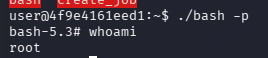
\includegraphics[keepaspectratio,alt={root}]{Vulnerabilities/Path 1/VPE/images/root.png}
        \end{center}

        As shown, we have successfully become root and this attack has been
        completed successfully.

    \newpage

    \section*{Path Bravo}
    Entering the Team Bravo section will lead to the following page:
    \begin{center}
        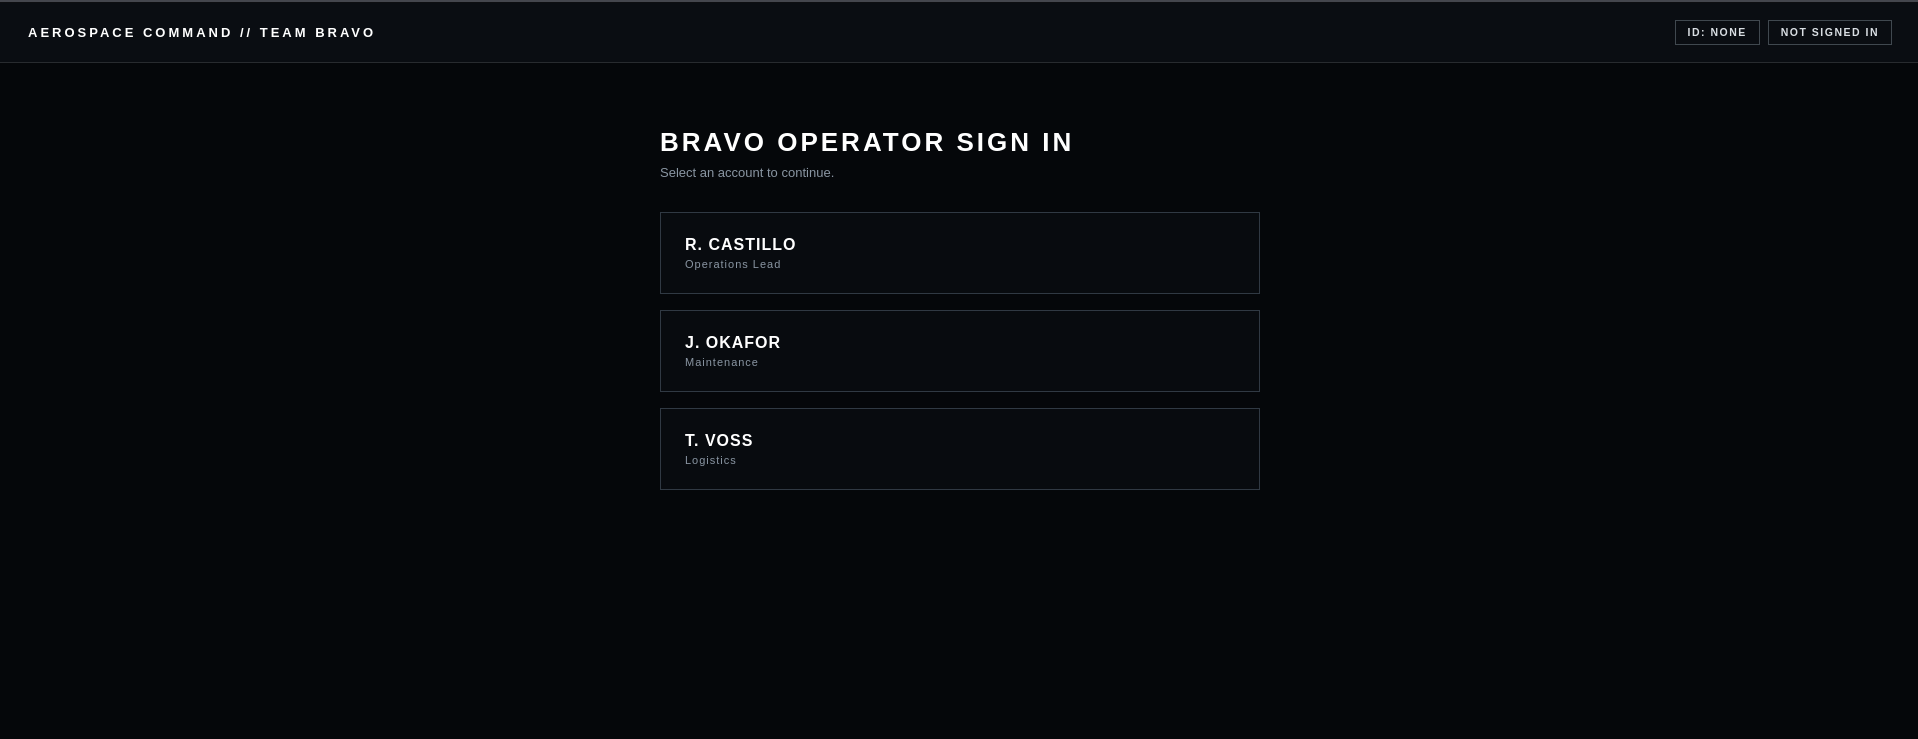
\includegraphics[scale=0.45]{Vulnerabilities/images/bravo.png}
    \end{center}

    \vspace{1em}

    \subsection*{Web (Mohammad)}

    \vspace{1em}

    \subsection*{Horizontal Privilege (Mohammad)}

    \vspace{1em}

    \subsection*{Web (Senaya)}

    \vspace{1em}

    \subsection*{Vertical Privilege (Senaya)}

    \newpage

    \section*{Path Charlie}
    Entering the Team Charlie section will lead to the following page:
    \begin{center}
        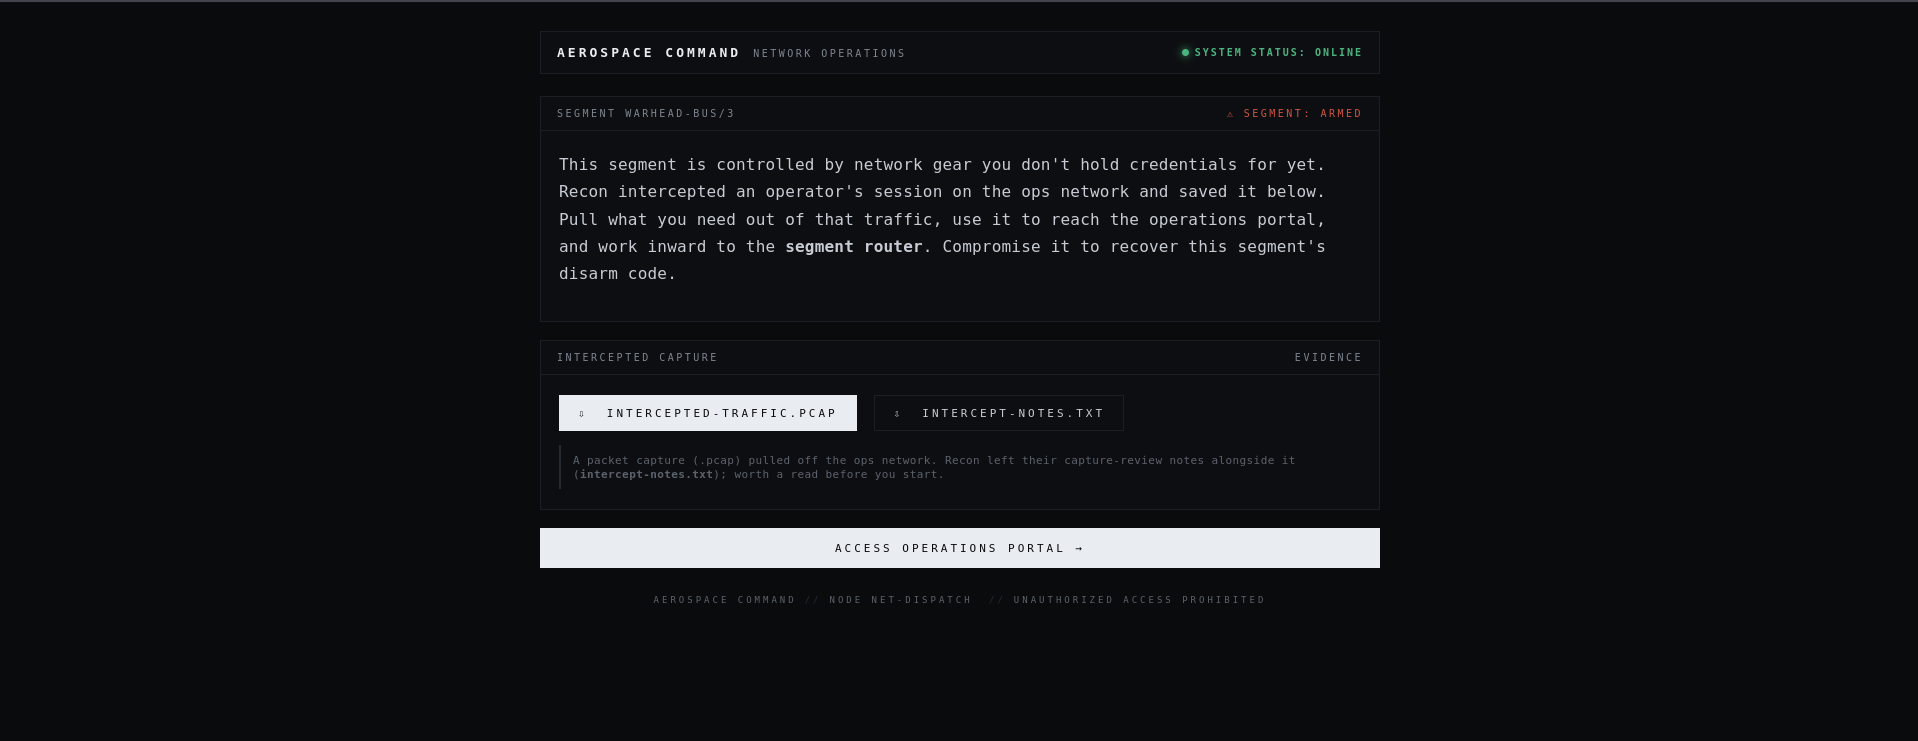
\includegraphics[scale=0.45]{Vulnerabilities/images/charlie.png}
    \end{center}

    This includes two downloadable files; \texttt{intercepted-traffic.pcap} and
    \texttt{intercept-notes.txt}, which are both necessary to complete the network
    challenge. These can both be downloaded to the local system to complete
    the challenge.

    \vspace{1em}

    \subsection*{Packet Analysis (Zarin)}
        The dashboard says that the operations portal needs some credentials
        that we don't currently have. Fortunately, the Recon team intercepted an
        operator's session and saved it. From here, we can inspect the
        intercepted session to try and get the credentials to log into the
        portal. The dashboard provides two files;
        \texttt{intercepted-traffic.pcap}, the intercepted session, and
        \texttt{intercept-notes.txt}, notes from the Recon team about the
        session. As these are both embedded downloads, we can download both of
        these to our host for further inspection. The notes are likely to hold
        information regarding what we should be looking for, so we should read
        this first.
        \begin{center}
            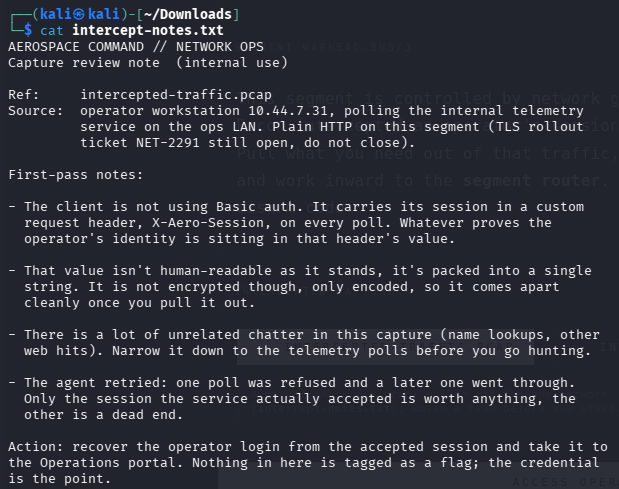
\includegraphics[keepaspectratio,alt={notes}]{Vulnerabilities/Path 3/Packet Capture/images/notes.png}
        \end{center}

        From these notes, we can gather a few bits of key information about
        where to look for the credentials: - It is being transmitted over HTTP -
        The auth token is stored in the \texttt{X-Aero-Session} header in every
        request - The value of the auth token is encoded in some format - The
        token is in the telemetry polls - There are two different requests to
        the telemetry polls where one went through and the other did not Using
        this information, we can now inspect the packet using Wireshark.
        \begin{center}
            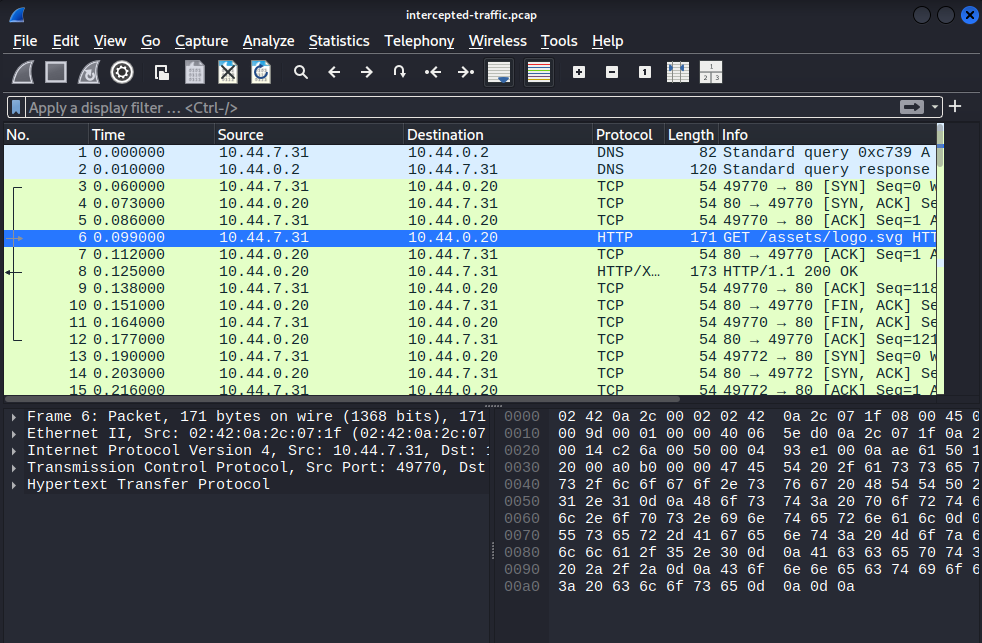
\includegraphics[scale=0.8]{Vulnerabilities/Path 3/Packet Capture/images/wireshark.png}
        \end{center}

        There is a lot of information here, so we can narrow it down according
        to the notes. As we know the credential is stored in a HTTP packet with
        the \texttt{X-Aero-Session} header, we can filter to only these packets
        with \texttt{http\ contains\ "X-Aero-Session"}.
        \begin{center}
            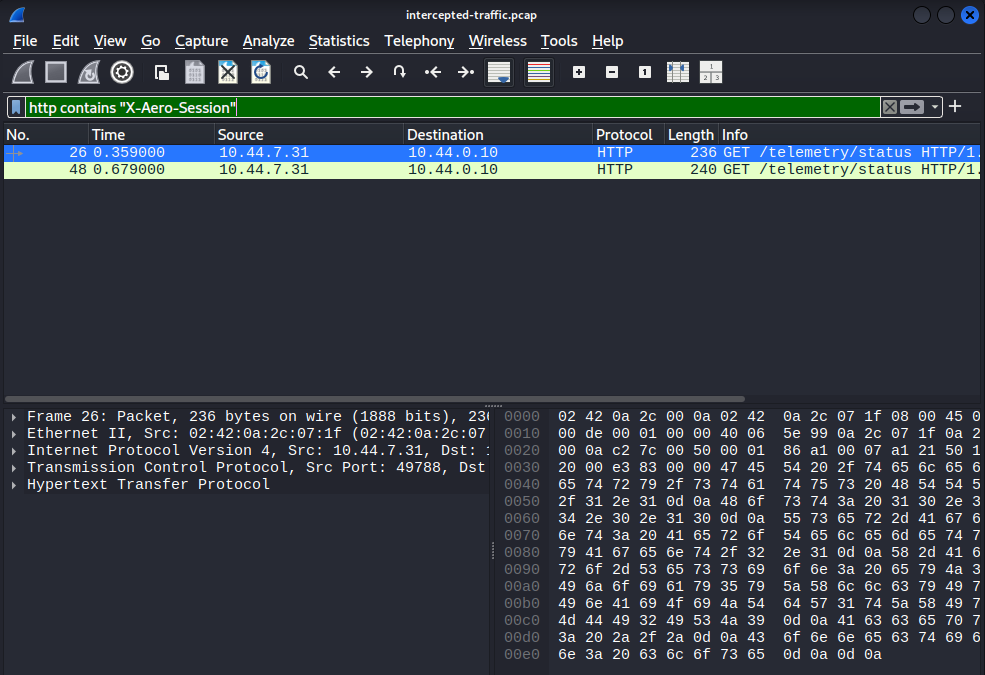
\includegraphics[scale=0.8]{Vulnerabilities/Path 3/Packet Capture/images/filter.png}
        \end{center}

        This has narrowed us down to two packets, which is just as the notes
        indicated. These both access \texttt{/telemetry/status}, so both need to
        be inspected to find the credential.
        \begin{center}
            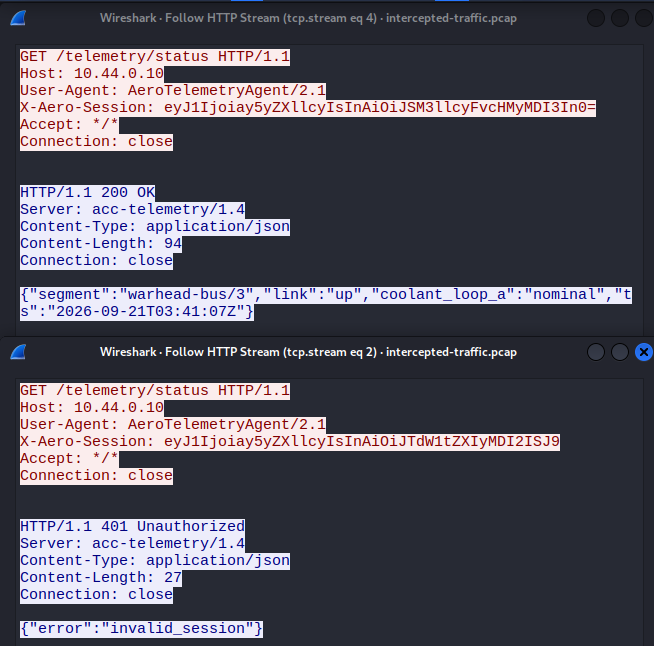
\includegraphics[scale=0.65]{Vulnerabilities/Path 3/Packet Capture/images/inspection.png}
        \end{center}

        It looks like the first request (\texttt{tcp.stream\ eq\ 4}) went
        through and the second request (\texttt{tcp.stream\ eq\ 2}) failed.
        Consequently, we can assume that the first request auth token
        (\texttt{eyJ1Ijoiay5yZXllcyIsInAiOiJSM3llcyFvcHMyMDI3In0=}) is the one
        we are looking for.

        Although we know that it is encoded, we don't know how it is encoded.
        However, there is an \texttt{=} sign at the end of the token. This is
        common with Base64 encoding, so we can try and decode it and see if we
        get anything. This can be done on our host using
        \texttt{echo\ eyJ1Ijoiay5yZXllcyIsInAiOiJSM3llcyFvcHMyMDI3In0\ \textbar{}\ base64\ -d}
        and looking at the output.
        \begin{center}
            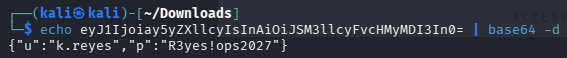
\includegraphics[keepaspectratio,alt={decode}]{Vulnerabilities/Path 3/Packet Capture/images/decode.png}
        \end{center}

        After decoding, it looks like the username is \texttt{k.reyes} and the
        password is \texttt{R3yes!ops2027}. Now that we have the username and
        password, we can try and sign into the operations portal using these
        credentials to see if they work.
        \begin{center}
            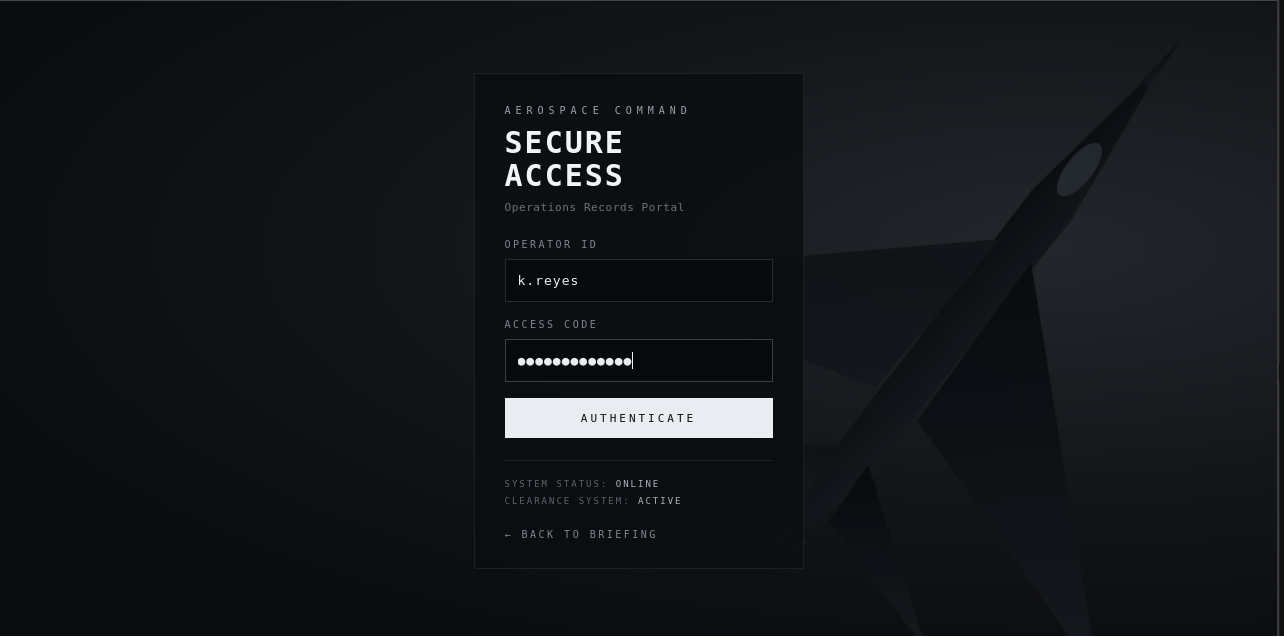
\includegraphics[scale=0.65]{Vulnerabilities/Path 3/Packet Capture/images/login.png}
        \end{center}

        After authenticating, these credentials were accepted and we are brought
        to an operations record panel.
        \begin{center}
            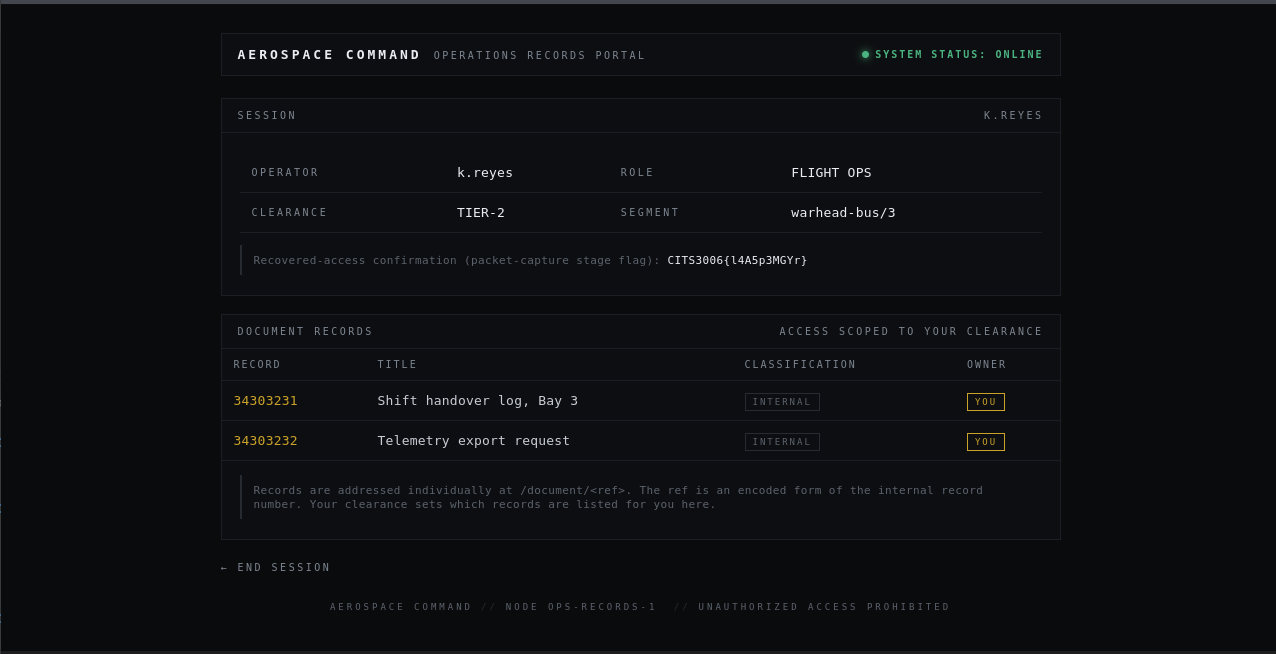
\includegraphics[scale=0.65]{Vulnerabilities/Path 3/Packet Capture/images/panel.png}
        \end{center}

        This has revealed the flag for the challenge, which is
        \texttt{CITS3006\{l4A5p3MGYr\}}.

    \vspace{1em}

    \subsection*{Insecure Direct Object Reference (IDOR) (Zarin)}
        The panel shows the document records for the current user, with the only
        two available being \texttt{34303231} and \texttt{34303232}. The panel
        says it is encoded, but does not specify the encoding so we need to do
        some more investigation. The first thing to try would be to read the
        documents available to see if they say anything of interest.
        \begin{center}
            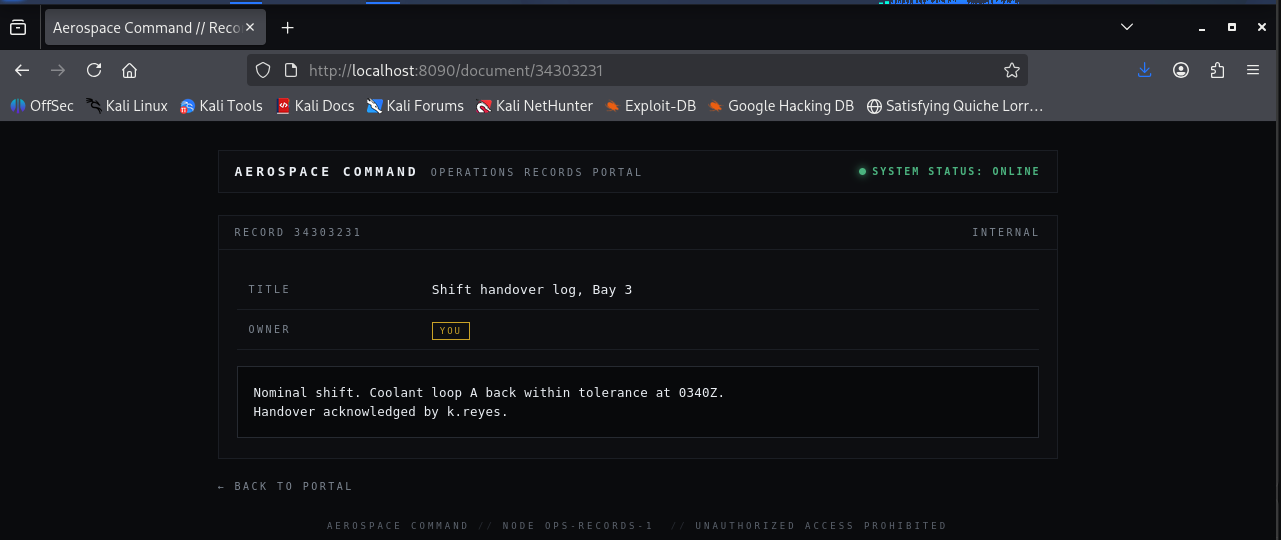
\includegraphics[scale=0.65]{Vulnerabilities/Path 3/HPE/images/34303231.png}
            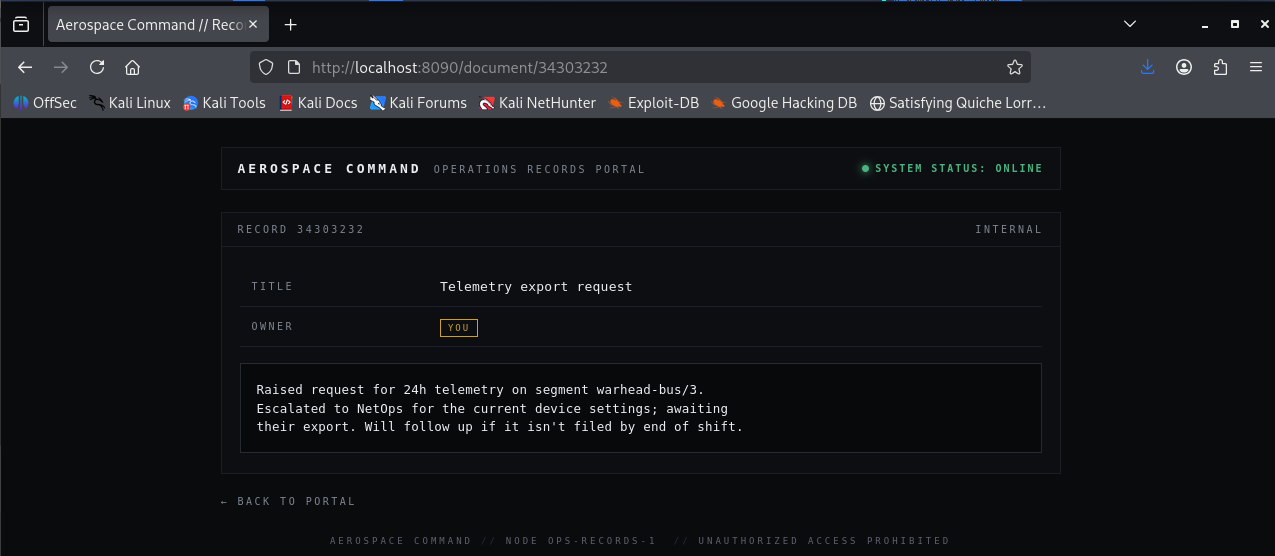
\includegraphics[scale=0.65]{Vulnerabilities/Path 3/HPE/images/34303232.png}
        \end{center}

        After reading the contents of both of these documents, there doesn't
        seem to be anything useful. However, the URLs for each document are
        interesting; they follow the
        \texttt{/document/\textless{}number\textgreater{}} format specified on
        the panel, so we may be able to try and look at other documents by
        changing this value. As a test, we can try and navigate to
        \texttt{/document/34303233} to see if there is any additional
        information we can get access to.
        \begin{center}
            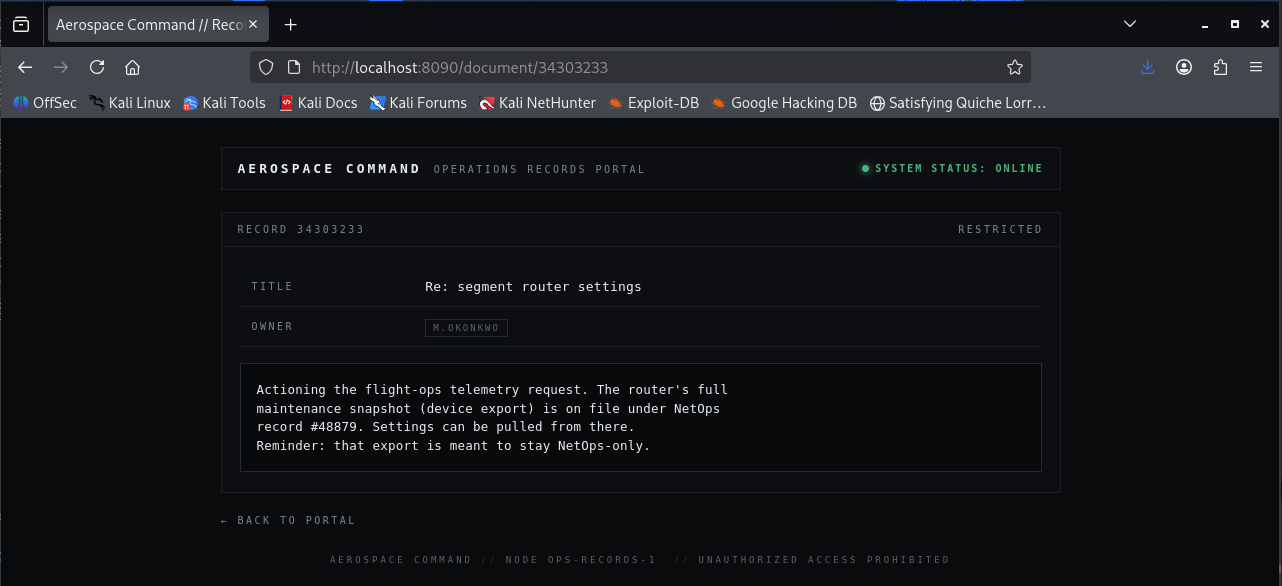
\includegraphics[scale=0.65]{Vulnerabilities/Path 3/HPE/images/34303233.png}
        \end{center}

        This has allowed us to view an additional document, despite it not being
        on our dashboard. This document specifically belongs to M. Okonkwo,
        meaning that our permissions aren't being checked when accessing
        documents which we may be able to take advantage of. This document
        specifically says that there is, supposedly, a maintenance snapshot for
        NetOps under document 48879. This is something we should probably look
        at, so let's try navigating to \texttt{/document/48879} to see if we can
        find anything.
        \begin{center}
            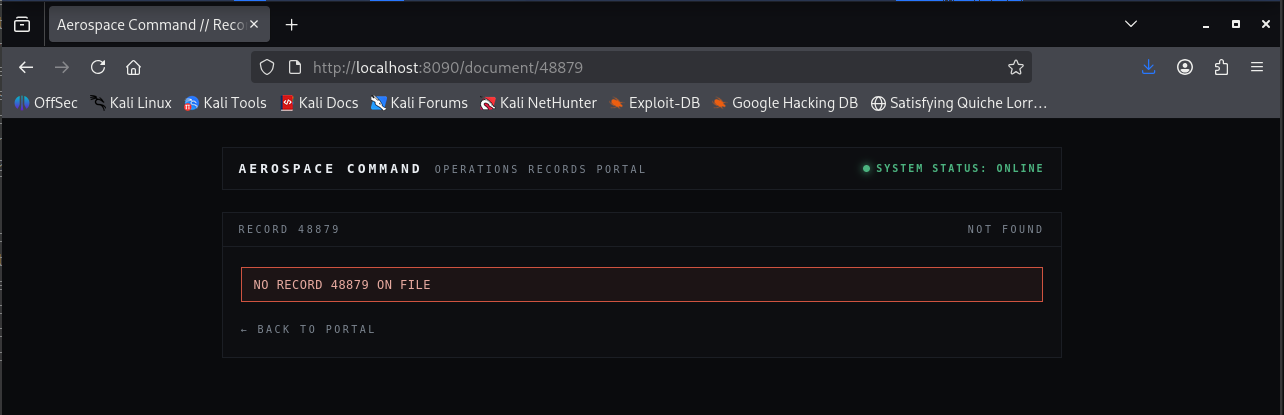
\includegraphics[scale=0.65]{Vulnerabilities/Path 3/HPE/images/48879.png}
        \end{center}

        This has returned that there is no results, so 48879 likely refers to
        the decoded number in the header. Therefore, we need to try and find
        what encoding scheme the URL uses to try and view this document. So far,
        all we know is that the document encoding can contain numbers which
        isn't very helpful as many encoding schemes can contain numbers.
        CyberChef contains many tools to encode and decode tools, so we can try
        different encoding schemes to see how this value is encoded and try to
        apply it to 44879.
        \begin{center}
            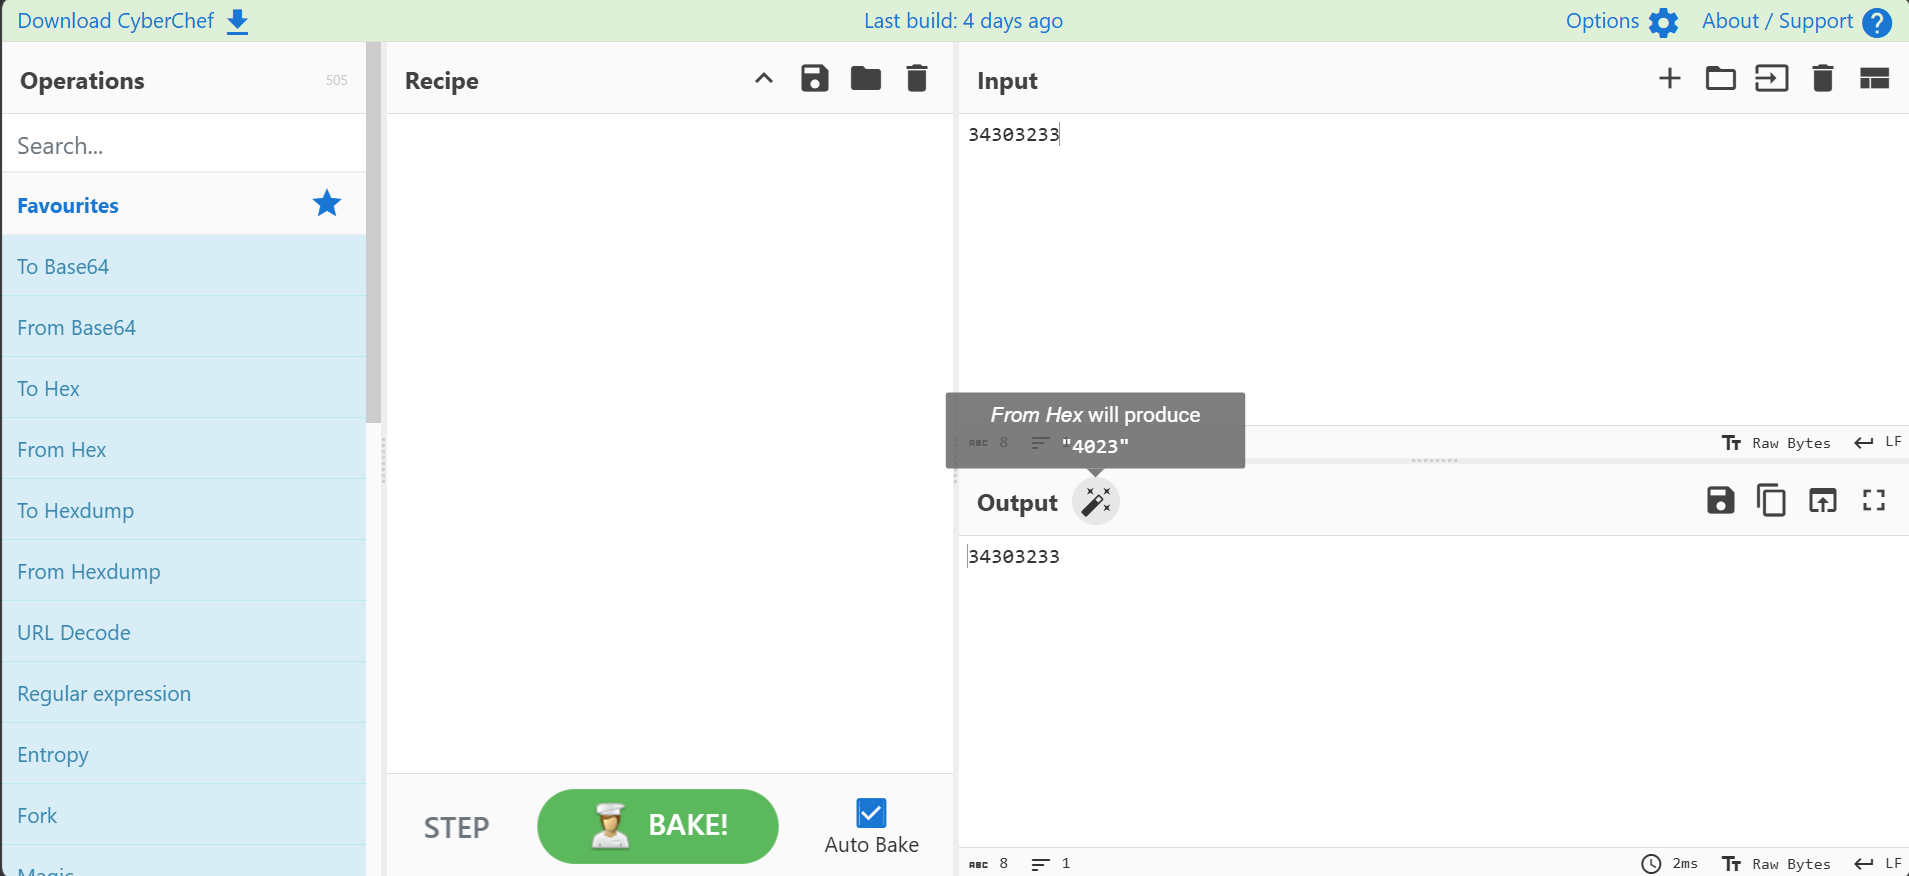
\includegraphics[scale=0.45]{Vulnerabilities/Path 3/HPE/images/cyberchef.png}
        \end{center}

        CyberChef has suggested to decode this value using Hex, which converts
        34303233 to 4023 (in decimal). This is worth exploring, so we need to
        convert 48879 to Hex and then attempt to use that as the URL
        parameter.
        \begin{center}
            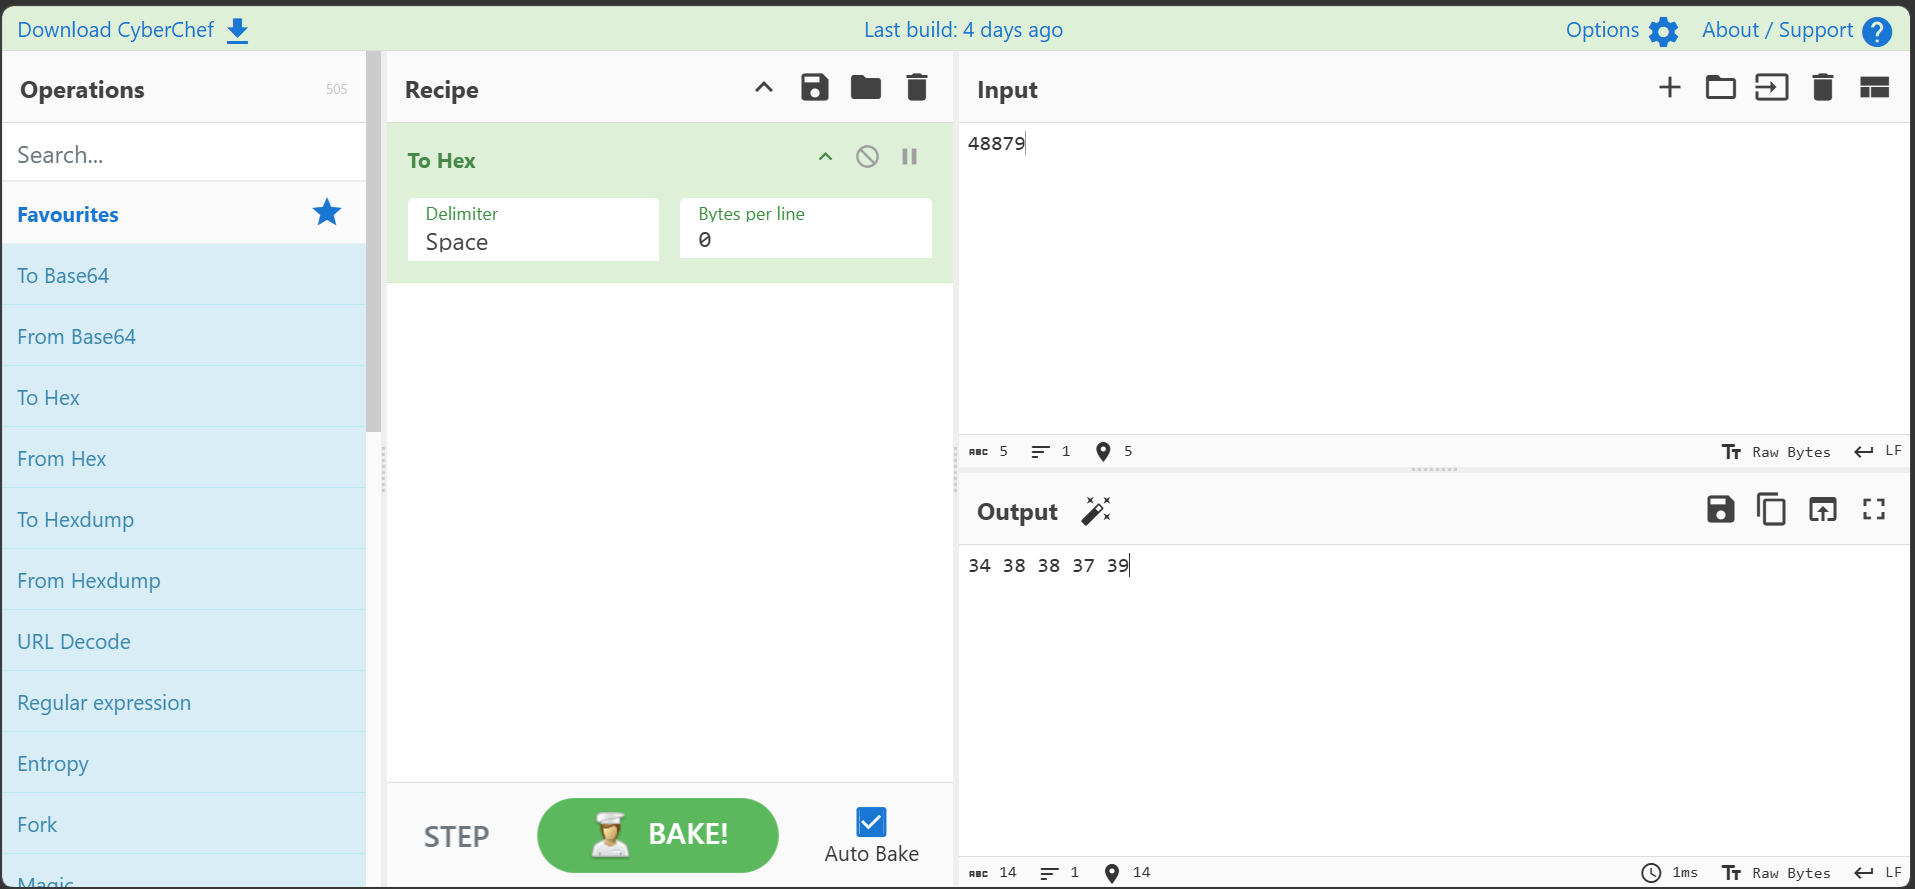
\includegraphics[scale=0.45]{Vulnerabilities/Path 3/HPE/images/conversion.png}
        \end{center}

        Converting 44879 to Hex has resulted in 34 38 38 37 39, or 3438383739
        which is a familiar format. Now all we need to do is try and access
        \texttt{/document/3438383739} and see if we get a result.
        \begin{center}
            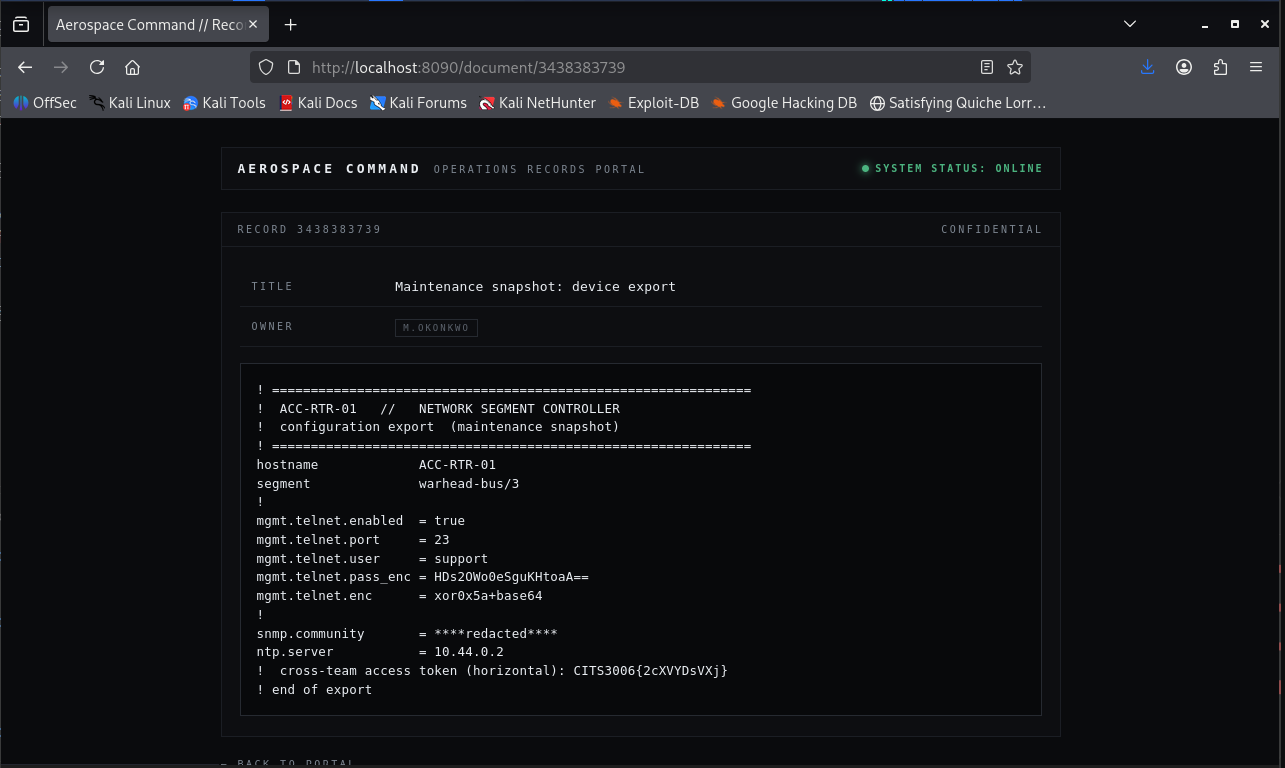
\includegraphics[scale=0.65]{Vulnerabilities/Path 3/HPE/images/escalation.png}
        \end{center}

        This has successfully retrieved the maintenance snapshot referred to
        earlier, which has a lot of information. Among this information is the
        flag for this challenge, which is \texttt{CITS3006\{2cXVYDsVXj\}}.

    \vspace{1em}

    \subsection*{Command Injection (Zarin)}
        Looking at the maintenance snapshot again indicates that the server has
        telnet enabled and provides some credentials to access it. Specifically,
        it lists the port number (\texttt{mgmt.telnet.port}), username
        (\texttt{mgmt.telnet.user}), and password
        (\texttt{mgmt.telnet.pass\_enc}) that are needed to connect to the
        machine. However, the password is encrypted which means we have to
        decrypt it. The snapshot appears to list the encryption scheme for the
        password (\texttt{mgmt.telnet.enc}), which it says uses
        \texttt{xor0x5a+base64}. As the password ends in \texttt{==}, we can
        assume that the base64 encoding was done last so this can be decoded to
        get the XOR'd password. This can be done using
        \texttt{echo\ HDs2OWo0eSguKHtoaA==\ \textbar{}\ base64\ -d\ \textbar{}\ xxd}
        to ensure that we aren't losing any bytes in the output.
        \begin{center}
            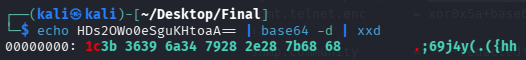
\includegraphics[keepaspectratio,alt={decode}]{Vulnerabilities/Path 3/Network/images/decode.png}
        \end{center}

        This output indicates that the Bash shell can't display one of the
        bytes, so the Base64 decoding needs to be done at the same time as the
        XORing to ensure that no bytes are lost (as otherwise the password will
        be incomplete). This can be done using Python, which has a native XOR
        operator and has the \texttt{base64} library as part of its standard
        library. The password can be recovered using
        \texttt{python3\ -c\ "import\ base64;\ print(\textquotesingle{}\textquotesingle{}.join(chr(b\^{}0x5A)\ for\ b\ in\ base64.b64decode(\textquotesingle{}HDs2OWo0eSguKHtoaA==\textquotesingle{})))"}.
        \begin{center}
            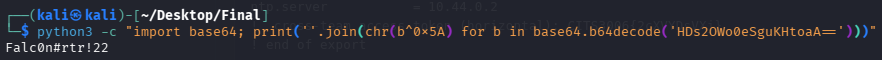
\includegraphics[keepaspectratio,alt={recovery}]{Vulnerabilities/Path 3/Network/images/recovery.png}
        \end{center}

        This has recovered the password \texttt{Falc0n\#rtr!22}, meaning we can
        now telnet into the server. Note that \texttt{localhost} is used instead
        of the container's IP below, but both should work the same.
        \begin{center}
            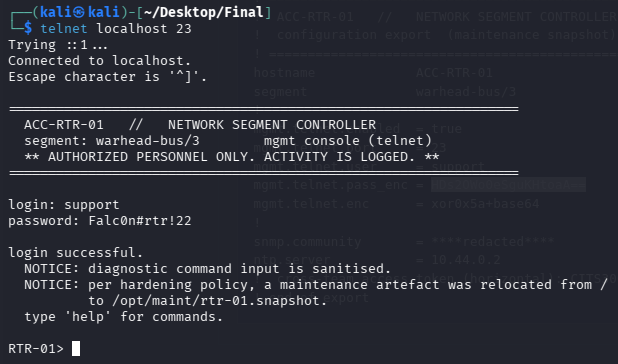
\includegraphics[keepaspectratio,alt={login}]{Vulnerabilities/Path 3/Network/images/login.png}
        \end{center}

        Now that we have logged into the machine, we can try and see what this
        is used for. There are two notices that are shown immediately upon
        login; one that indicates command input is sanitised, and another that
        indicates that some sort of maintenance artefact is located at
        \texttt{/opt/maint/rtr-01.snapshot}. As this was done for security
        hardening purposes, this file likely contains private information which
        we may be able to use. We don't know what commands we have access to, so
        we need to list them with \texttt{help}.
        \begin{center}
            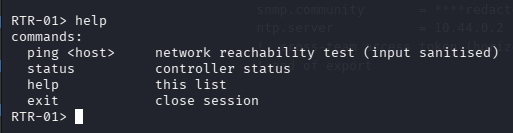
\includegraphics[keepaspectratio,alt={help}]{Vulnerabilities/Path 3/Network/images/help.png}
        \end{center}

        It looks like the only commands we have access to are \texttt{ping},
        \texttt{status}, \texttt{help}, and \texttt{exit}. \texttt{help} and
        \texttt{exit} won't be helpful to us (this is shown after using
        \texttt{help} and leaving won't get us anywhere) so we need to look at
        \texttt{ping} and \texttt{status}. It looks like \texttt{ping} is input
        sanitised, so it is likely that this has some sort of exploit. As a
        test, we can see what the \texttt{ping} command returns when given
        random data since this is likely how we are able to read that
        maintenance file identified earlier.
        \begin{center}
            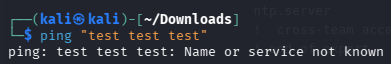
\includegraphics[keepaspectratio,alt={test\_ping}]{Vulnerabilities/Path 3/Network/images/ping_test.png}
        \end{center}

        It looks like \texttt{ping} will print whatever text is passed to it if
        it cannot resolve it to an IP address, meaning we may be able to use it
        to print the contents of the maintance file. We need to see how this
        \texttt{ping} command works before we do anything else.
        \begin{center}
            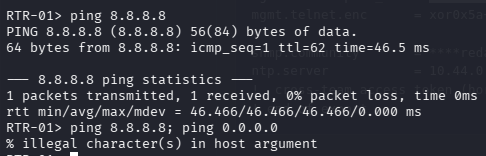
\includegraphics[keepaspectratio,alt={test\_sanitisation}]{Vulnerabilities/Path 3/Network/images/test_sanitisation.png}
        \end{center}

        After trying to chain multiple \texttt{ping} commands together, the
        input sanitisation was triggered. This likely means that the commands
        are being processed by some shell, which could possibly expand our
        available options. To confirm that the commands are, in fact, being
        processed by a shell interpreter, we can craft a payload to cause the
        shell to error rather than the \texttt{ping} command. This can be done
        simply using an open bracket (i.e.~\texttt{ping\ (}), which should cause
        the shell to error.
        \begin{center}
            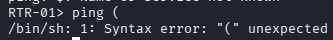
\includegraphics[keepaspectratio,alt={shell}]{Vulnerabilities/Path 3/Network/images/shell.png}
        \end{center}

        As suspected, the commands are being processed by a shell (and more
        specifically by \texttt{bash}). This means that we can potentially read
        the file by using \texttt{cat} on the maintenance file in a subshell,
        since \texttt{bash} will expand the subshell before executing
        \texttt{ping}. We can try this by running
        \texttt{ping\ \$(cat\ /opt/maint/rtr-01.snapshot)}, which should
        hopefully read the file.
        \begin{center}
            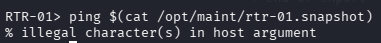
\includegraphics[keepaspectratio,alt={subshell}]{Vulnerabilities/Path 3/Network/images/subshell.png}
        \end{center}

        This has resulted in an invalid character being detected, so we need to
        figure out which one is being blocked. We know that brackets are already
        accepted, so we just need to test \texttt{\$} and \texttt{}.
        \begin{center}
            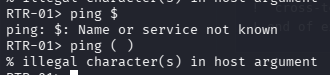
\includegraphics[keepaspectratio,alt={illegal}]{Vulnerabilities/Path 3/Network/images/illegal.png}
        \end{center}

        Unexpectedly, it seems like \texttt{} is the invalid character.
        Fortunately, there is an easy solution for this; \texttt{bash} has a
        special shell variable called \texttt{IFS} (or Internal Field Separator)
        that can be used to represent whitespace. Although it is typically used
        for word-splitting, we can use it act as whitespace to run this command.
        This can be done using
        \texttt{ping\ \$(cat\$\{IFS\}/opt/maint/rtr-01.snapshot)}.
        \begin{center}
            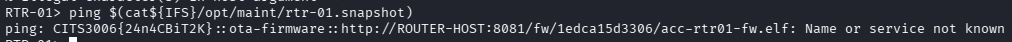
\includegraphics[scale=0.9]{Vulnerabilities/Path 3/Network/images/finale.png}
        \end{center}

        This has printed the contents of the file, allowing us to see that the
        flag for this challenge is \texttt{CITS3006\{24n4CBiT2K\}}.

    \vspace{1em}

    \subsection*{\texttt{rbp} Manipulation (Isaac)}
        Looking at the output of the maintenance file, we can see that it says
        \texttt{ota-firmware::http://ROUTER-HOST:8081\\/fw/1edca15d3306/acc-rtr01-fw.elf}.
        This seems to indicate that some sort of firmware is stored at
        \texttt{http://ROUTER-HOST:8081/fw/1edca15d3306/acc-rtr01-fw.elf}, which
        we can download onto our host using
        \texttt{wget\ http://localhost:8081/fw/1edca15d3306/acc-rtr01-fw.elf}.
        \begin{center}
            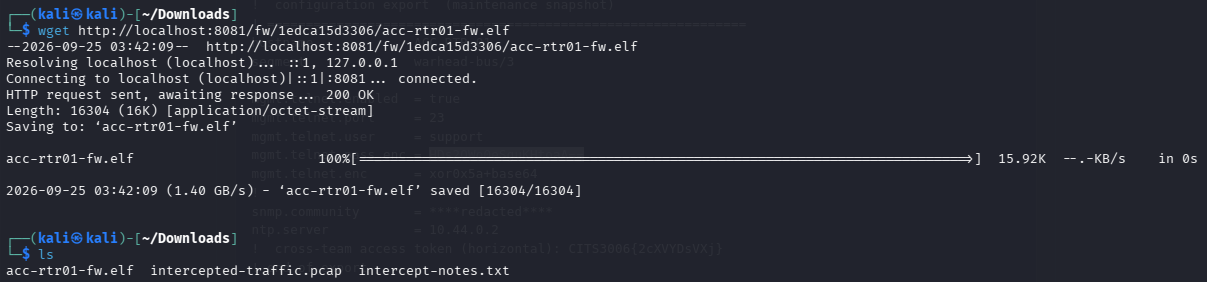
\includegraphics[scale=0.75]{Vulnerabilities/Path 3/RE/images/wget.png}
        \end{center}

        Before we do anything, the binary will be renamed to \texttt{bin} so
        that it is easier to interact with in the shell.
        \begin{center}
            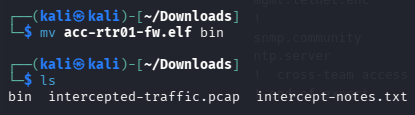
\includegraphics[keepaspectratio,alt={rename}]{Vulnerabilities/Path 3/RE/images/rename.png}
        \end{center}

        Now that we have the binary on our system, we can inspect it to see what
        it does. We can see what it does by calling \texttt{./bin} after making
        sure it is executable with \texttt{chmod\ +x\ bin}.
        \begin{center}
            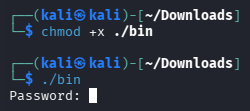
\includegraphics[keepaspectratio,alt={bin}]{Vulnerabilities/Path 3/RE/images/bin.png}
        \end{center}   

        The program is asking us for some sort of password, which we obviously
        don't have. However, we should see what it does given input anyway since
        that could guide us to what we have to do.
        \begin{center}
            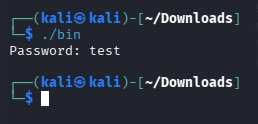
\includegraphics[keepaspectratio,alt={test}]{Vulnerabilities/Path 3/RE/images/test.png}
        \end{center}

        After trying a random password, the program literally returns nothing.
        We can try to check any embedded strings in the program using
        \texttt{strings\ bin}, which may contain the password for the binary in
        plaintext.
        \begin{center}
            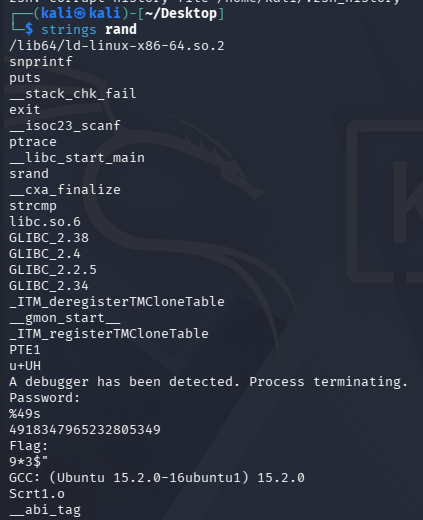
\includegraphics[scale=0.7]{Vulnerabilities/Path 3/RE/images/strings.png}
        \end{center}

        The strings seem to primarily be referencing functions, but there are
        some notable strings that can be seen in the binary. There's the
        password entry text, a random string of numbers
        (\texttt{4918347965232805349}), and a piece of string that seems to
        imply that the flag is printed somewhere (but likely obfuscated in some
        form). The string of numbers is interesting, and could be the password
        so we can try it and see what happens.
        \begin{center}
            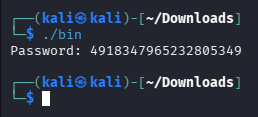
\includegraphics[keepaspectratio,alt={failed}]{Vulnerabilities/Path 3/RE/images/failed_password.png}
        \end{center}

        This has also caused nothing to happen, so we need to investigate
        something else. We can also inspect the properties of the binary using
        \texttt{file\ bin}, which may have something that can be exploited.
        \begin{center}
            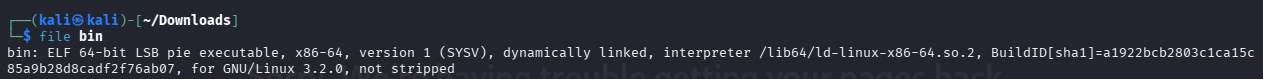
\includegraphics[scale=0.65]{Vulnerabilities/Path 3/RE/images/file.png}
        \end{center}

        This appears to be a fairly standard binary. However, it is dynamically
        linked meaning that libraries are loaded at runtime instead of at
        compile time. This means it could potentially be vulnerable to an
        \texttt{LD\_PRELOAD} attack, but we have to find a function that can be
        bypassed to actually exploit this. It is also unstripped, meaning that we
        may be able to view function names through a debugger. Since we have
        access to the binary on our local machine, we can attach it to a
        debugger (like \texttt{gef}) to see how it works internally and identify
        any functions which could be bypassed using this method.
        \begin{center}
            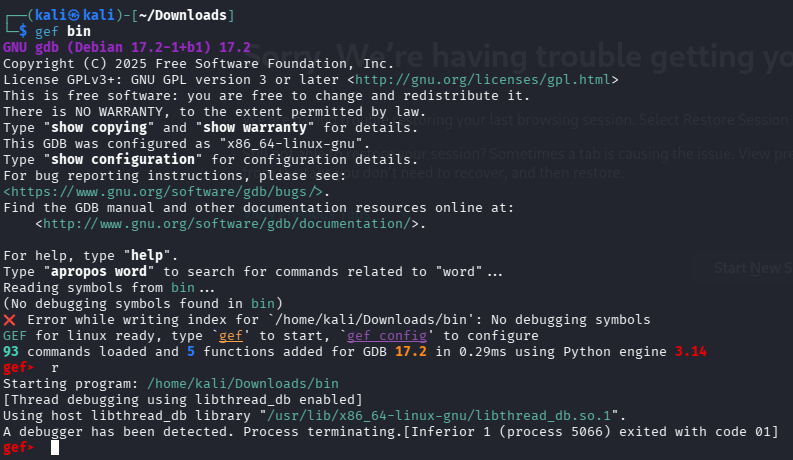
\includegraphics[keepaspectratio,alt={debugger}]{Vulnerabilities/Path 3/RE/images/debugger.png}
        \end{center}

        After attempting to run it with the debugger, it leads to an error. It
        is likely using some anti-debugger technique to prevent it being run in
        debuggers, which we can check using \texttt{disas\ main}.
        \begin{center}
            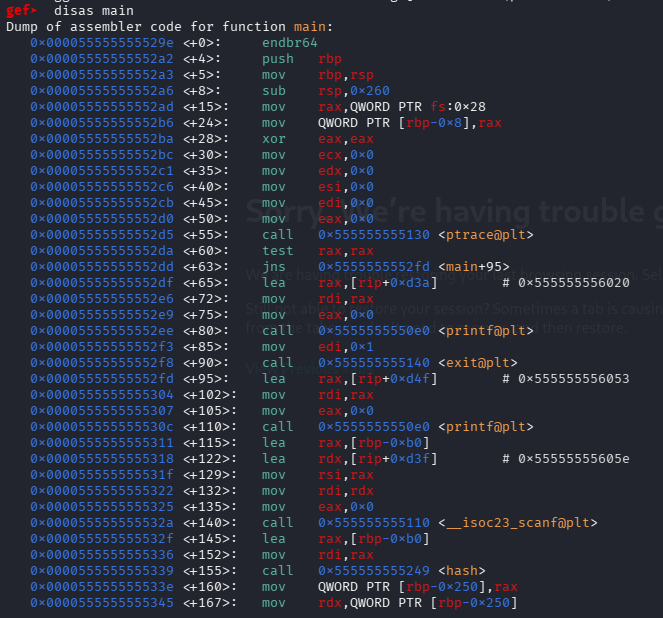
\includegraphics[scale=0.75]{Vulnerabilities/Path 3/RE/images/disas_main.png}
        \end{center}

        This disassembly has shown a \texttt{ptrace} function call, which is
        commonly used to prevent programs being debugged. By taking advantage of
        the fact that this binary is dynamically linked, we can write a custom
        implementation of this function that allows us to bypass this check
        entirely. All this needs to do is return 0, and can be written like the
        following:

        \begin{verbatim}
        long ptrace(int request, int pid, void *addr, void *data) {
            return 0;
        }
        \end{verbatim}

        To make this available as a shared library, it can be compiled as
        \texttt{gcc\ -shared\ ptrace.c\ -o\ ptrace.so}.
        \begin{center}
            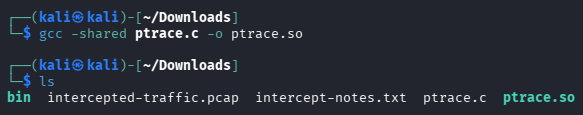
\includegraphics[keepaspectratio,alt={shared}]{Vulnerabilities/Path 3/RE/images/shared.png}
        \end{center}

        Now that the library has been compiled, we can load it when we start
        running the program. This can be put into the environment using
        \texttt{set\ environment\ LD\_PRELOAD=./ptrace.so}, which will cause any
        \texttt{ptrace()} call to use this function instead.
        \begin{center}
            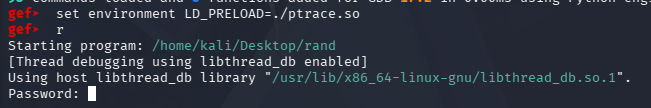
\includegraphics[keepaspectratio,alt={bypass}]{Vulnerabilities/Path 3/RE/images/bypass.png}
        \end{center}

        Now that we have access to the program, we can investigate it further.
        We still don't know what the password is, so we need to find some
        further information. As we know the binary isn't stripped, we can have a
        look at some of the functions the binary includes.
        \begin{center}
            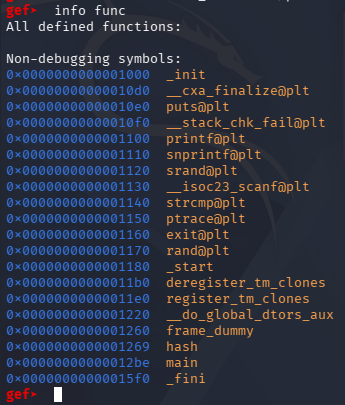
\includegraphics[keepaspectratio,alt={functions}]{Vulnerabilities/Path 3/RE/images/functions.png}
        \end{center}

        These are all C and system functions, with the exceptions of
        \texttt{main} and \texttt{hash}. \texttt{main} isn't interesting since
        all standlone C binaries will include one, but \texttt{hash} is
        interesting and likely indicates that the password is hashed before
        being checked. We don't expect \texttt{hash} to contain any useful
        information since it just sounds like a hashing function, so exploring
        \texttt{main} again will be the next step. Just to make it easier, this
        will be done using Ghidra.
        \begin{center}
            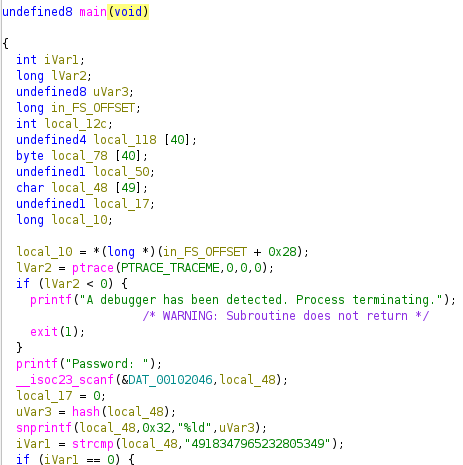
\includegraphics[keepaspectratio,alt={decompiled}]{Vulnerabilities/Path 3/RE/images/decompiled_main.png}
        \end{center}

        This decompilation of \texttt{main} produced by Ghidra has a few points
        of interest: - The \texttt{ptrace} call terminates program execution if
        it succeeds - The input is hashed and passed as a string - The hash is
        compared to \texttt{4918347965232805349} (which is the string identified
        earlier) To make viewing this decompilation easier, the variables can be
        renamed.
        \begin{center}
            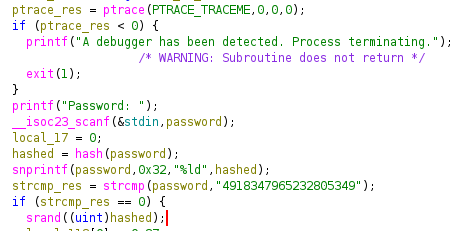
\includegraphics[keepaspectratio,alt={clean}]{Vulnerabilities/Path 3/RE/images/decompiled_main_clean.png}
        \end{center}

        After cleaning up the decompilation, it seems like the hash value is
        used to seed a random number generator using \texttt{srand}. To confirm
        this, we need toenter this branch which we can do by finding a password
        that hashes to the value \texttt{4918347965232805349}. Although this
        could be brute forced, this will take a long time; instead, we can use
        \texttt{gef} to insert this value into memory just before the string
        comparison to enter this branch. This requires looking at the
        disassembled \texttt{main} function identify where the password input is
        stored in memory so we can adjust its value directly.
        \begin{center}
            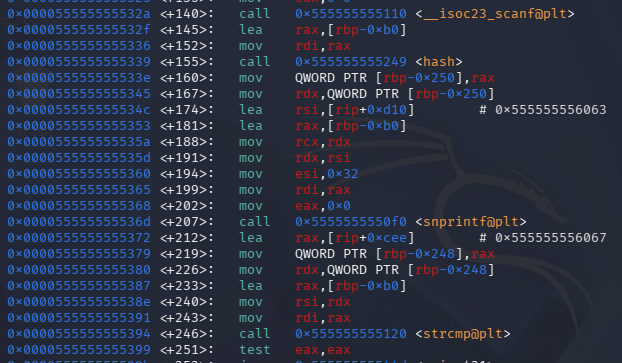
\includegraphics[keepaspectratio,alt={scanf}]{Vulnerabilities/Path 3/RE/images/gef_scanf.png}
        \end{center}

        At various points, there are a few addresses that have data being
        transferred into them: - \texttt{rbp\ -\ 0xb0} - \texttt{rbp\ -\ 0x250}
        - \texttt{rbp\ -\ 0x248}

        The one that sticks out the most is in the instructions before the
        \texttt{hash} function is called. The \texttt{lea} instruction is used
        to move the memory held in \texttt{rbp\ -\ 0xb0} to the \texttt{rax}
        register. This is then moved to the \texttt{rdi} register, which is
        where the first argument for functions is stored. As the \texttt{hash}
        function is called directly afterwards, this seems like the perfect
        candidate for where password input is stored. To confirm this, a
        breakpoint can be placed just before the \texttt{hash} function (using
        \texttt{b\ *0x555555555249}) and the \texttt{rdi} register inspected.
        \begin{center}
            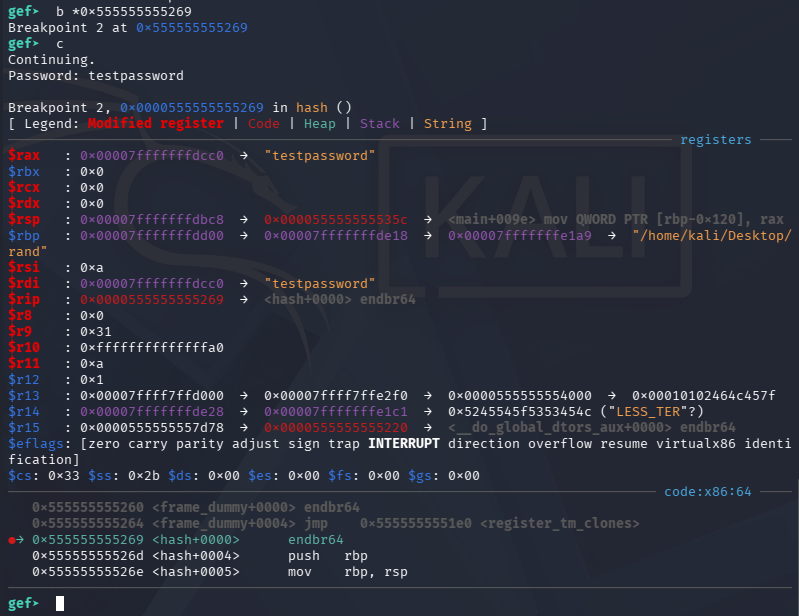
\includegraphics[scale=0.8]{Vulnerabilities/Path 3/RE/images/rdi.png}
        \end{center}

        As expected, the \texttt{rdi} register (and \texttt{rax} register)
        contains the input password. Therefore, the input password is contained
        at \texttt{rbp\ -\ 0xb0}. We can utilise this fact to force this memory
        to be the hash value, bypassing the need to find the password entirely.
        This can be done by setting a breakpoint at the \texttt{strcmp}
        instruction (using \texttt{b\ *0x0000555555555391}), changing the value
        of \texttt{rbp\ -\ 0xb0} to the ``correct'' hash value using
        \texttt{set\ \{char{[}20{]}\}(\$rbp-0xb0)\ =\ "4918347965232805349"},
        and then continuing function execution.
        \begin{center}
            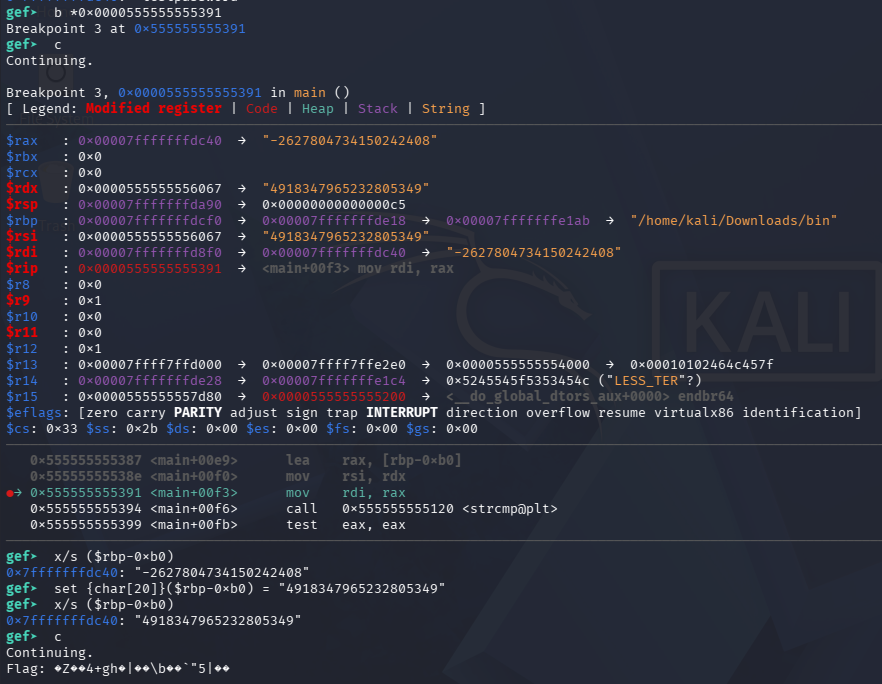
\includegraphics[scale=0.75]{Vulnerabilities/Path 3/RE/images/rbp-0xb0.png}
        \end{center}

        As shown, this has actually allowed program execution to continue within
        the branch but the output does not look as expected. This probably has
        something to do with the random seed identified earlier, which uses the
        hashed value as the seed. Since changing the value at \texttt{rbp-0xb0}
        only changed the string representation, we also need to change the value
        of the hash value itself. In the earlier disassembled code,
        \texttt{rbp-0x250} seems like a good candidate since that is the value
        accessed directly after the \texttt{hash} function returns so we can
        inspect that.
        \begin{center}
            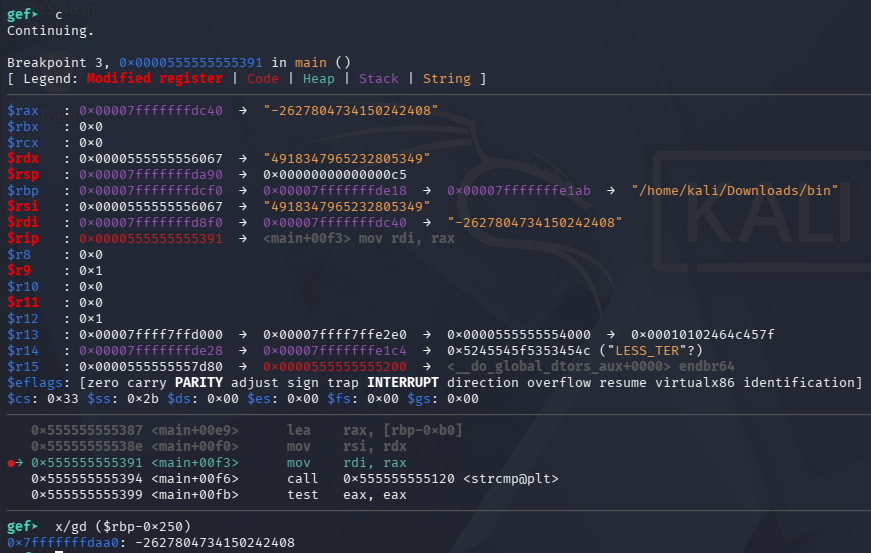
\includegraphics[scale=0.75]{Vulnerabilities/Path 3/RE/images/rbp-0x250.png}
        \end{center}

        As shown, the address at \texttt{rbp\ -\ 0x250} holds the exact same
        value (in decimal) as \texttt{rdi} which, in this case, is the string
        representation of the hash of the password input. As such, it can be
        changed using
        \texttt{set\ \{long\}(\$rbp\ -\ 0x250)\ =\ 4918347965232805349} to
        ensure that both \texttt{rbp\ -\ 0x250} and \texttt{rbp\ -\ 0xb0} hold
        the same value. If both of these are changed and the program execution
        continues, the following results:
        \begin{center}
            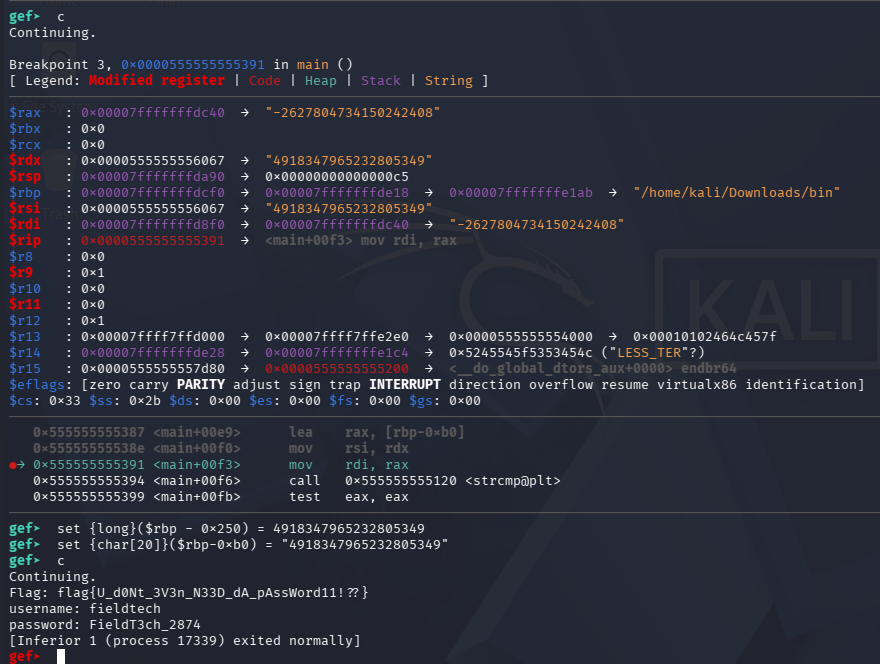
\includegraphics[scale=0.75]{Vulnerabilities/Path 3/RE/images/finish.png}
        \end{center}

        This has revealed the flag, which is
        \texttt{flag\{U\_d0Nt\_3V3n\_N33D\_dA\_pAssWord11!??\}}. Some
        credentials have also been revealed, which will be required to complete
        the next challenge.

    \vspace{1em}

    \subsection*{Sudo \texttt{NOPASSWD} Misconfiguration (Zarin)}
        Now that we have some credentials, we can use them to access the server.
        This is done with SSH, which listens on port 2022.
        \begin{center}
            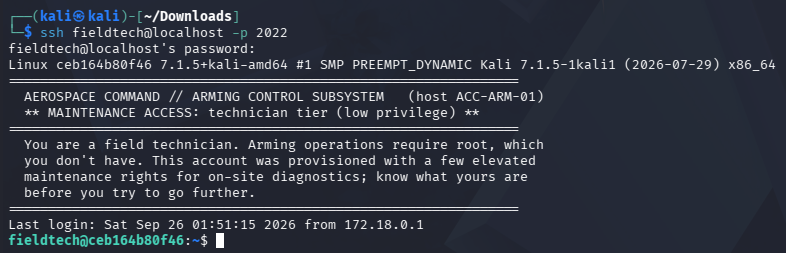
\includegraphics[keepaspectratio,alt={login}]{Vulnerabilities/Path 3/VPE/images/login.png}
        \end{center}

        Now that we have signed in, we need to perform reconnaissance. The entry
        message says that we have ``a few elevated maintenance rights'' so we
        should check what we have access to. This involves checking the
        permissions of files in our home directory (with \texttt{ls\ -al}),
        looking for any setuid binaries (with
        \texttt{find\ /\ -type\ f\ -perm\ -4000\ 2\textgreater{}/dev/null}),
        looking for any capabilities (with
        \texttt{getcap\ -r\ /\ 2\textgreater{}/dev/null}), and looking for any
        binaries we can run as root (with \texttt{sudo\ -l}).
        \begin{center}
            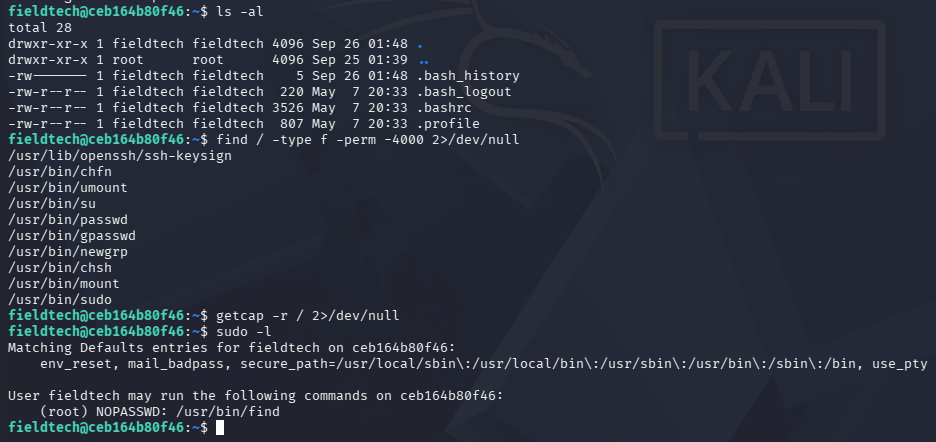
\includegraphics[scale=0.8]{Vulnerabilities/Path 3/VPE/images/privileges.png}
        \end{center}

        There isn't anything interesting in our home directory, but it looks
        like there are a few binaries with the setuid bit enabled and a single
        binary (\texttt{find}) that can be run using \texttt{sudo} with no
        password. This is actually the most interesting one, and is worth
        exploring further. We can look at what command line arguments it accepts
        using \texttt{find\ -\/-help}, as it may have something that can be
        exploited.
        \begin{center}
            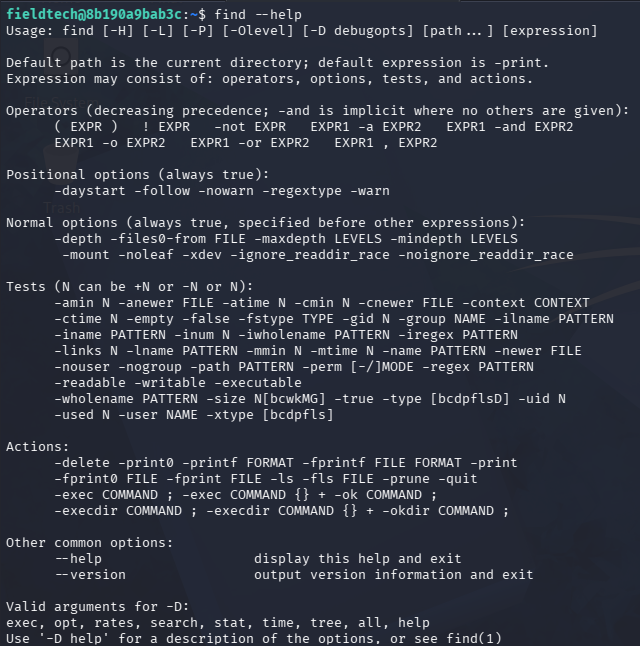
\includegraphics[scale=0.8]{Vulnerabilities/Path 3/VPE/images/help.png}
        \end{center}

        It looks like it supports an \texttt{-exec} flag, which can seemingly
        run arbitrary commands. We can test this out by crafting a payload that
        causes the command to run \texttt{/bin/bash}, which should give us a
        root shell when running with \texttt{sudo} (as \texttt{sudo} makes it
        run as root and no password is required to run \texttt{find} using
        \texttt{sudo}). This only needs to be a simple payload that follows this
        command's conventions, so
        \texttt{sudo\ find\ -exec\ /bin/bash\ \textbackslash{};} should
        hopefully work.
        \begin{center}
            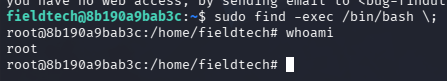
\includegraphics[keepaspectratio,alt={exec}]{Vulnerabilities/Path 3/VPE/images/exec.png}
        \end{center}

        This has given us a root shell, meaning this attack has been completed
        successfully.

        \newpage

        \section*{Individual Contributions}
            \dots
\end{document}
